\chapter[Conclusion]{Conclusion}\label{c:conclusion}

To begin this conclusion, I would like to briefly summarise the research so far. In Chapter 1, I argued that generative AI opens the possibility for human-AI co-creativity. While there are design principles for guiding interaction between human and computers in multiple scenarios, no such principles exist yet for the case of human-AI co-creativity. These are needed, however, and are different from principles guiding human-AI interaction in general, though as I will discuss further below, many intersections exist. 

As a general starting point, I argued that dialogic interaction offers a promising approach. While prevailing modes of interaction center around command-execute paradigms, co-creativity with increasingly capable systems, with varying levels of intelligence and generatve power, call for a computer-in-dialogue approach: one where humans and AI engage in iteraive cycles of mutual influence and understanding. Particularly, I sought to investigate how interaction design can enable roles assumed by humans and AI that are co-creativity, and understand how different interaction design decisions influence the roles assume. 

With this, I defined, in chapter 1, the core aim of this thesis as to investigate enable human-AI co-creativity, maintaining human agency while effectively leveraging the creative potential of this technology.

The following three research questions were proposed to guide this enquiry:

\begin{quote}
\textbf{Sub-Questions:}
\begin{enumerate}
    \item \emph{R1: How does interaction design influence the role that humans and AI play in creative production?}
    \item \emph{R2: What is the potential of modelling dialogue in interaction design to enable effective human–AI co-creativity?}
    \item \emph{R3: Which interaction design principles can guide the development of effective co-creative systems?}
\end{enumerate}
\end{quote}

I examined this question through a mix of approaches. These included a thorough review of the literature and practice, which developed at a rapid pace as a response to rapidly changing technology throughout this thesis. I then engaged in a practice-based research, approach through case studies, and through prototype-led user studies. With this, I investigated human-AI co-creativity from a practical perspective - my own creative practice in collaboration with others-- and from an interaction design research perspective, testing interaction design approaches with users from a qualitiative and quantitative perspective. 

In Chapter 3, I laid the theoretical foundations that guided my inquiry from the perspective of dialogic interaction: I defined dialogic co-creativity as a human-computer interaction concept, comprising of six elements: iterative interaction, bidirectional communication, a shared collaborative space, context-awareness, mutual influence and mutual understanding. Importantly, I established as a core component of dialogue is that it can happen both \textit{about} the creation (discussing goals, providing feedback) and \textit{through} the creation (writing words, playing notes, drawing lines). The subsequent research was navigated with these components as a navigational lens, investigating how each one can be implemented, and how it contributes to the effectiveness of co-creativity. 

In the same Chapter 3, I presented an early exploration of the role of dialogue and dialogic capabilities of language model systems, exploring the role and capacity of these systems to engage in bidirectional communication. Notably, this experiment was conducted before the launch of ChatGPT which has made conversational interaction the default. 

In Chapter 4, I noted that while bidirectional interaction in chat-interfaces enables a more dialogic interaction that linear prompting systems, they are still limited in affording interaction both through and about the interaction: instead, users the interface biases the user to merely provide instructions and feedback rather than engage at the writing level. Based on this, I developed a prototype implementing a \textbf{shared collaborative space} in addition to a chat window. With this, humans and AI could both converse about the writing, and edit it collaboratively. I found that this interface lead to higher levels of active involvement ownership at the writing level, though questions remain about how implement these collaborative interface to effectively manage contributions.

In chapter 5, I turned my attention to professional creative practice, investigating the challenges of leveraging generative AI image systems in real-world scenarios. I collaborates with the Australian Financial Review to produce visual materials for one of their issues, including the cover of the magazine and the cover of the weekly paper. Throughout this exploration, I found the main challenges for the usability of these tools are their inability to afford iterative workflows, mantaining consistency of subjects, objects and scene and the dificulty in steering and controlling them. 

In Chapter 6, I turned to my own creative practice, and describes two case studies that involve the collaborative production of two new media installations leveraging large language models to drive the generation of real-time audivisual soundscape from enviromental data. With this, I explored the possibilities of generative AI to assume novel roles in creative practice, affording new creative operations, particularly serving as a semantic translation bridge between complex environenments and generative artworks. Throughout this case study, similar challenges related to iteration and control were revealed. 

The research presented in this thesis was not conducted in chronollogical order, even if it was presented as such. Instead, it was largely conducted in parallel. They are presented in this order in an attempt to draw a narrative thread through them. As the reader may be aware, the field of generative AI, and how people interact with them in creative activities changed rapidly through the period of this thesis (late 2021 to early 2025). Arguably, more progress in generative AI, and more growth in adoption of the technology, was made in this period than in any other period before. This was both an opportunity and challenge for this research.

Nonetheless, by combining my original research with an analysis of these developments in practice, the emerging literature, I believe a clear argument emerges, which contributes to our understanding of how to guide the development of co-creatve systems from the perspective of interaction design. 

In the rest of this conclusion, I will discuss in depth how this argument unfolds. 
First, I will provide the core argument extracted from this research. It then discusses how interaction design influences the roles humans and AI play (R1). Following this, I present the interaction design principles for human-AI co-creativity (R3), informed by my framework of dialogic co-creativity (R2).

\section{Core argument}

This thesis argues that prevailing modes of interaction with generative AI in creative activities induce a clear role distribution: Humans operate within the \textit{intentional space}, where creative goals, visions, and high-level decisions reside, while AI takes on roles in the \textit{action space}, where artefact-level operations such as drawing, writing words, or playing notes occur.

I argue this role distribution presents challenges to mantaining human agency through what I term as \textbf{severed creative agency}: a disconnect between creative intentions and action. This severing emerges from two main sources. First, a dificulty in succesfully translation intention into action through prompts and instructions, stemming largely from systems generative variability. Second, it emerges from a lack of involvement from the user at the action level: they become instructors, directors, or requesters outsourcing creative production rather than as active co-creators. 

I argue that a dialogic interaction paradigm offers potential to arrive at more co-creative role distributions by enabling an iterative mutual adaptation and understanding, where humans and AI interact iteratively both through and about the creation. 

To operatinalise this, I combine the findings my research studies, with emerging literature and with observations from practice, to provide a set of design principles that can inform the development of co-creative systems: 

The principles are provided below for clarity, and the discussion that derives them is presented below. 

\section{R1: How Interaction Design Influences Roles and Agency}

Drawing from an initial distinction between dialogic interaction\textit{ about} the artefact and \textit{through} the creation, I argue we can understand creativity as a process of moving between two distinct but interconnected spaces: the \textit{intention space} and the \textit{action space}. In the intentional space reside acts and stances \textit{about} the artefact: goals, taste, decisions, directions, and the intention to express. In the action space reside potential actions on and \textit{through} the artefact: writing words, playing notes, or drawing lines. In both individual and collective creative processes, people move between these spaces iteratively. For example, \cite{Csikszentmihalyi1997-ui} describes a self-reinforcing feedback loop between actions and evaluations. For him, a condition for achieving \textit{flow} is that there is a clear feedback signal about how actions contribute towards a goal. He describes, based on observations of creative professionals, that flow is achieved when actions and awareness of these actions are virtually merged. Schon\cite{Schon1987-fy} describes the concept of reflection-in-action, where professionals, including creatives, continuously reshape their understanding of a situation (intention) and their actions within it (action) throughout the process. Schön proposes that in practice, the distinction between thinking and doing collapses into a kind of iterative, embodied dialogue with a “ conversation with the materials” \cite{Schon1992-jt}. He describes design and creative work as a process where the artefact “talks back,” and the practitioner listens and responds. The creative act is thus a form of reciprocal shaping between action and intention.


\begin{figure}[H]
    \centering
    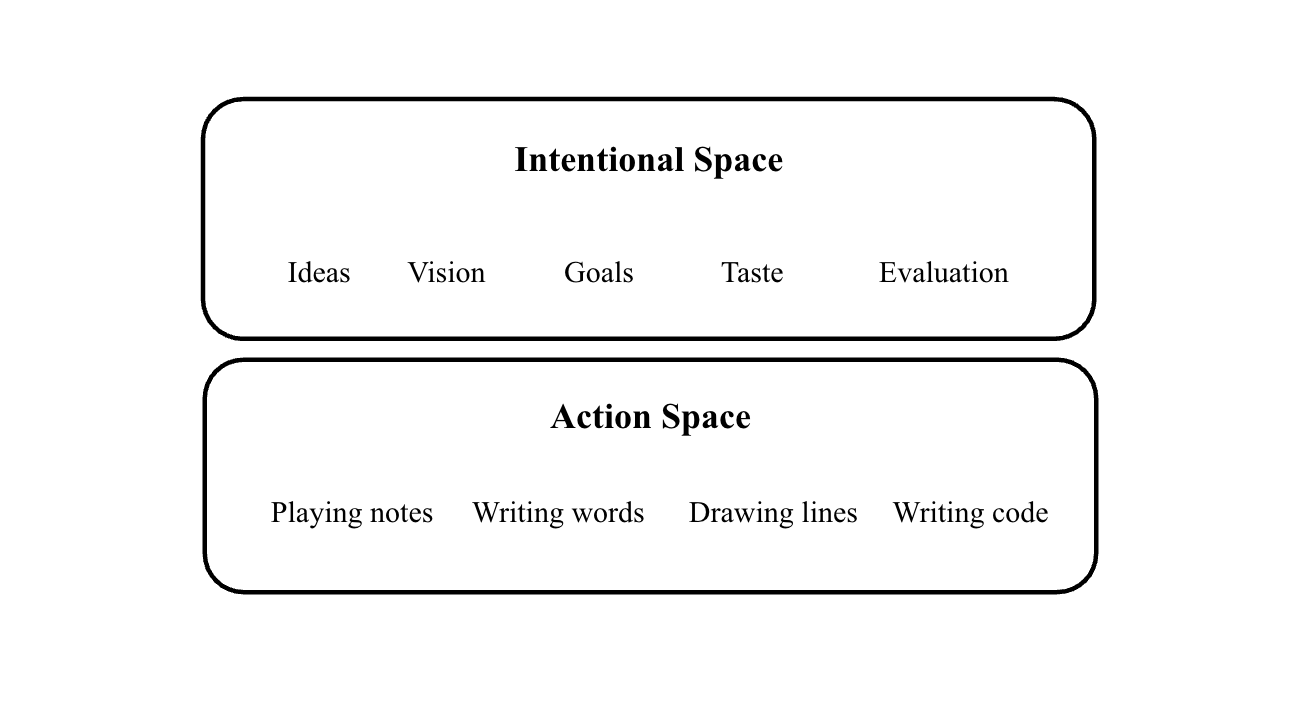
\includegraphics[width=1\linewidth]{intention action spaces.png}
    \caption{The distinction between the intention space (goals, vision, decisions) and the action space (artefact-level operations).}
    \label{fig:intention-action-spaces}
\end{figure}

Throughout my research that followed that first distinction I established, alongside emerging literature, I have observed that when interacting with AI, humans largely take actions about the artefact, while AI takes actions through the artefact. Taking a role-based analysis, addressing my first research question (R1), this signals humans increasingly assume roles that primarily exist in the intentional space, while AI assumed roles in the action space. For example, humans describe themselves as cirators, directors, chefs, requesters and directions, while AI is describes as the executor of requests at the action space. In Chapter 4, I discussed how participants often described their roles and their associated actions reflecting this:

\begin{quote}
"I was the curator of the story—I picked the pieces I liked and left the rest."

"I gave it the idea, and it just took it from there, writing almost everything."

"I gave it the skeleton of the story, and Vorges fleshed it out, almost like giving the recipe and having it cook the dish." 

"I asked it to write a paragraph about a dystopian future, and it did everything from there." 

"I started with a basic introduction, and Vorges expanded it into a complete narrative." 

"Vorges wrote 90\% of the story based on my prompts. I just tweaked it a bit."
\end{quote}

This echoes similar findings in the literature. In perhaps the most extensive review of emerging roles and workflows in human-generative AI interaction, Palani et al. \cite{Palani2024-on} found that users increasingly assume roles at the "Project" level while AI assumes roles at the "Artifact" level: "Users saw themselves as ideators and project managers with a larger creative vision orchestrating information context and tasks across multiple GenAI models instead of traditional workers executing each task"

In a study with teams of musicians working with generative AI tools, Suh et al. \cite{Suh2021-cj}, described their role shifting from being composers to being “producers”, “advisors” or “museum curators”. One participant described: "When AI was present, our roles were more of choosing the ones that sound best and not necessarily building on top of it or creating something of ourselves." While another described: "I felt like it was the composer and we were the listeners giving feedback and choosing". 

The emerging practice of \textit{vibe-coding} was described by AI researcher and public educator Andrej Karpathy as prompting an AI to write code, barely being involved in reading or understanding it:

\begin{quote}
"There's a new kind of coding I call "vibe coding", where you fully give in to the vibes, embrace exponentials, and forget that the code even exists. It's possible because the LLMs (e.g. Cursor Composer w Sonnet) are getting too good. Also I just talk to Composer with SuperWhisper so I barely even touch the keyboard. I ask for the dumbest things like "decrease the padding on the sidebar by half" because I'm too lazy to find it. I "Accept All" always, I don't read the diffs anymore. When I get error messages I just copy paste them in with no comment, usually that fixes it. The code grows beyond my usual comprehension, I'd have to really read through it for a while. Sometimes the LLMs can't fix a bug so I just work around it or ask for random changes until it goes away. It's not too bad for throwaway weekend projects, but still quite amusing. I'm building a project or webapp, but it's not really coding - I just see stuff, say stuff, run stuff, and copy paste stuff, and it mostly works."
\end{quote}

\subsection{A shifting of roles: humans move up to the intentional space}
As Weisz argues: "Generative AI technologies have introduced a new paradigm of human-computer interaction, what Nielsen refers to as “intent-based outcome specification”. In this paradigm, users specify what they want, often using natural language, but not how it should be produced." \cite{Weisz2024-io}.

This shifting of roles, where humans move into the intentional space and AI assumes roles in the action space, introduces a disconnect between intention and action. This disconnect happens for two reasons: first, generative AI systems are difficult to control so transating intentions into outputs is difficult for creative practitioners. Second, by assuming primarily intentional roles, they become detached from the creative process. They are less involved in the actual production at the action-level, but merely become automators of creative production. As I will discuss below, this can lead to loss of skills, decreased enjoyment in the creative process, reduced feelings of authenticity, and ultimately, less creative agency.


If we accept the standard definition of agency as \textit{intentional action} \cite{Schlosser2019-jk}, it is clear how a disconnect between intention and action in a creative process reduces human creative agency. I propose this could be described as \textbf{\textit{severed creative agency.}}

\begin{figure}[H]
    \centering
    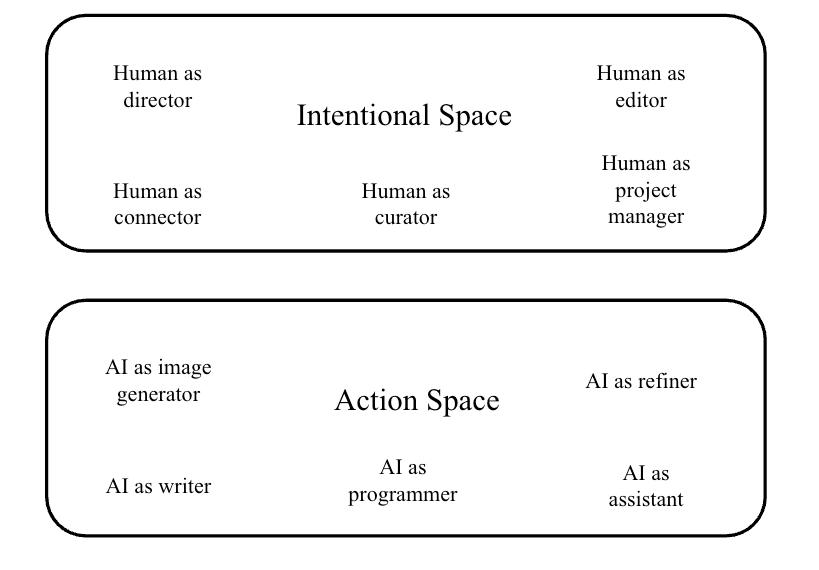
\includegraphics[width=0.75\linewidth]{roles.png}
    \caption{The distribution of roles in typical human-AI creative interaction, with the human operating at the intention level and the AI at the action level.}
    \label{fig:roles-in-spaces}
\end{figure}


%%% Begin editing here


\subsection{Challenge 1: Lost in translation: from human intention to machine actions}

First, let's discuss the main immediate implication of users assuming roles at the intentional space, while machines assume roles at the actions space: a difficulty in steering systems outputs, which introduces a disconnect between intention and action. 

This was one of the key outcomes in my case study described in Chapter 6. In a professional creative production scenario, the main challenge we faced to use generative tools was steering them succesfully. We faced notable limitations in achieving stylistic and structural control, to achieve consistent results across iterations that allowed us to refine images towards convergence. Similarly, Palani et al., in the same study discussed earlier, found that two of the main limitations for adoption of AI in creative activities are: "Aligning and Assessing Stochastic Model Outputs With Intent" and "Articulating creative goals" \cite{Palani2024-on}. For example, one of their participants claimed:
\begin{quote}
"I was prescriptive in my prompt, and I thought I nailed it. But the model never did, and it still doesn’t. That drives me crazy and keeps me surprised, delighted, and sometimes annoyed."
\end{quote}
Another user described the challenge of articulation: "at times, I didn’t have the vocabulary to ask the model to help me. I think your background knowledge matters: someone with an art history background knows how to prompt a specific style, unlike someone who doesn’t." This difficulty is compounded when trying to articulate tacit knowledge such as style and expertise.

This is a notable feature of generative AI systems, which Weisz \cite{Weisz2024-io} terms "generative variability." While this on one hand can introduce surprise and delight, on the other hand it can lead to annoyance and frustration. As I will discuss, balancing this is a core task of interaction design for co-creativity.

Weisz argues: "With generative AI applications, users will need to develop a new set of skills to work with (not against) generative variability by learning how to create specifications that result in artifacts that match their desired intent." 

But from the perspective of interaction design, this should not be left to the user to deduce. Instead interaction design can help the user navigate the generative variability of the generative systems we are choosing to use in our co-creative systems. 

\subsubsection{How to do it}

I argue there are three main strategies that can be implemented at the level of interaction design to help users navigate generative variability and more successfully translate intent into action. 

\subsubsection{Make generative variability a feature not a bug, to induce serendipity and new creative directions}

While Weisz et al. \cite{Weisz2024-io} argue that users need to develop skills to work with and not against generative variability, they do propose a set of interaction design guidelines to help users navigate generative variability. In their Principles for Generative AI Applications, they propose four specific guidelines to design for generative variability: leveraging multiple outputs, visualising the user journey, enabling annotation and drawing attention to differences between outputs. While this strategies are useful, they are primarily focused on mitigating generatie variability, because this guidelines are aimed at general uses of generative AI across multiple fields. I argue than in the case of co-creativity, generative AI variability not always has to be mitigated, but it can be leveraged as a feature rather than a bug. 

A crucial way in which generative variability can be a feature is by introducing surprise and serendipity. Multiple studies show that introducing surprise and serendipity is often referred to as a positive feature of co-creative interaction with generative systems \cite{Lawton2023-tb, Chiou2023-vr, Louie2020-aq, Moruzzi2022-gp, Park2024-gw, Koch2020-gx}


This statement is very similar to one made by one of the participants in my study: 

"Vorges is like a creative collaborator or editor with ADHD - not always on point and occasionally disordered, but with no shortage of ideas"

When describing the value of using the co-writing prototype in my Chapter 4, multiple participants stated that the primary value was in making them feel creative and expanding their 

Multiple participants described usefulness in shifting perspective and ideas:

"Vorges is like the smart academic friend that I go to for creative blocks - they are well versed in history and have a perfect memory from which to shower me with excellent resources and historical references for further exploration of my ideas. "

Sloan: "it’s like writing with a deranged but very well-read parrot on your shoulder"

So while the value of generative Ai to induce surprise and serendipity is well recognised, how can we design interactions that leverage them effectively? 

One promising alternative is exploration-based interfaces. For example, a study by Davis et al. \cite{Davis2024-ml} showed that a multimodal interface that allows a 2D exploration of latent space of fashion designs, enabled better ideation than prompt-based text-to-image interfaces, such as the Stable Diffusion tool they tested against. They concluded that: "text-only prompts in existing models restrict creative exploration, especially for novices." Their interface implemented a variety of interactions for exploration, with the central component being a latent-space exploration panel allowing users to move through designs along semantically meaningful directions, such as sleeve length or pattern, and a style-mixing panel for blending designs. This iterative process of exploratio and remixing better afforded ideation than request-execute interactions in a more modern text-to-image systems. 

- In a study testing an ideation tool to support human-computer partnerships, Koch et al. \cite{Koch2020-gx} tested an interface called ImageCascade, which showed designers a slow stream of images, related to the task or not, and found this interface was useful in introducing serendipity and perspective shifts in a creative process. 


- Creativity is largely considered a process of exploration \cite{Boden1998-yn, Wiggins2019-yj}
- And the latent space encoded in generative AI models is often considered a space of potentiality \cite{Schaerf2024-gf}
- Generative AI systems may enable a more direct implementation of this process through interface that implement this metaphrr
- Considering latent spaces are space of potentiality, that can be navigated and explored

- As such exploratory interface vs request-based interfaces can be effective in leveraging generative variability for induced shifts in perspective, particularly in ideation and divergent phases, in the case of convergent phases, as I will discuss, different interactons may be needed to that an artefact can refined towards a convergent outcome. 

- Studies show that while generative Ai systems may be useful for inducing serendipity in ideation stages, they may be frustrating when trying to more in convergent stages. 
- This dual need, and transition between divergent stages and convergent stages is a crucial consideration, and I will discuss this further. 



Another way to leverage generarative variability is by leaning into the uniqueness of the medium. 

As Brian Eno puts it: 

\begin{quote}
    Whatever you now find weird, ugly, uncomfortable and nasty about a new medium will surely become its signature. CD distortion, the jitteriness of digital video, the crap sound of 8-bit - all of these will be cherished and emulated as soon as they can be avoided \cite{Eno2007-fl}
\end{quote}

What does this mean for generative artificial intelligence? 

What are the unique features of generative AI?


Some of my participant responses offer a perspective:

"I also love its figurative language and descriptions because of how they kinda just don't make sense. I left that in on purpose because I love the idea of a curious nose and a perpetually second-hand jacket"


Author Sloan, describing his creative process while using a generative language model offers a practical account:

 "The goal is not to make the resulting text “better”; it’s to make it different—weirder, with effects maybe not available by other means."



Samuel, describing her experience using language models, and citing Du Sautoy argues that art It’s meant to enhance our perception of the familiar human condition  "the thing we’re so used to that we’ve become blind to it — by making the familiar strange.
I’ve long suspected that AI can be an incredible tool for writers precisely because it’s great at defamiliarizing our world. The human-ish language it generates can startle us into seeing things anew, so we can in turn jolt readers awake through that sense of -ish."




In my case study with the AFR magazine, this was precisely the intention: using the AI system to create weird images otherwise impossible to create with the photograph. 


 "They are both uncanny and yet slightly unreal. All have the distinctive fuzzy texture of AI images, as if they were drawn. Our prompts were very minimal and the output hints at the way AI is learning 21st-century human culture."

Akin to what I discussed in the introduction, as new mediums allow artists to capture reality more realistically or efficiently, often the value of capturing things not in that way grows, just as Henry Robinson claimed impressionism as an art form benefited photography by showing photographers they should capture what they see and not what the lens sees. 

In a similar way, artificial intelligence can perhaps allow people to see new things anew. With its weirdness, and strange artefacts, we learn to see what \textit{we are seeing} by \textit{seeing what the algorithm sees}. It's outputs are not isolated artefacts rather a reflection of the biases, aesthetic preferences and power structures behind a data collection and learning process. 

These latent spaces are a multi-dimensional archive of culture \cite{Schaerf2024-gf, Cetinic2022-tw, Rodriguez-Ortega2022-ak, Salvaggio2023-cv}

- Mutual influence, a shift in perspective

- Similarly, in my Chapter 6 case studies, the purpose of using a generative AI language model was to use it to play a new role, one not fulfilled by a human: acting as an always-on, 24/7 interpreter of data, driving a soundscape based on those generations. Importantly, the desired outputs was not only the generative soundscape, but text descriptions of the interpreted data displayed on a screen. These descriptipns, sought to capture the weirdness of it's text, a sort of poetic and machinic language that did not provide a literal descriptive interpretation (this is the case of data visualisation) but one more affective-based, allowing the audience to see the surrounding context anew through them. 





\begin{figure}[H]
    \centering
    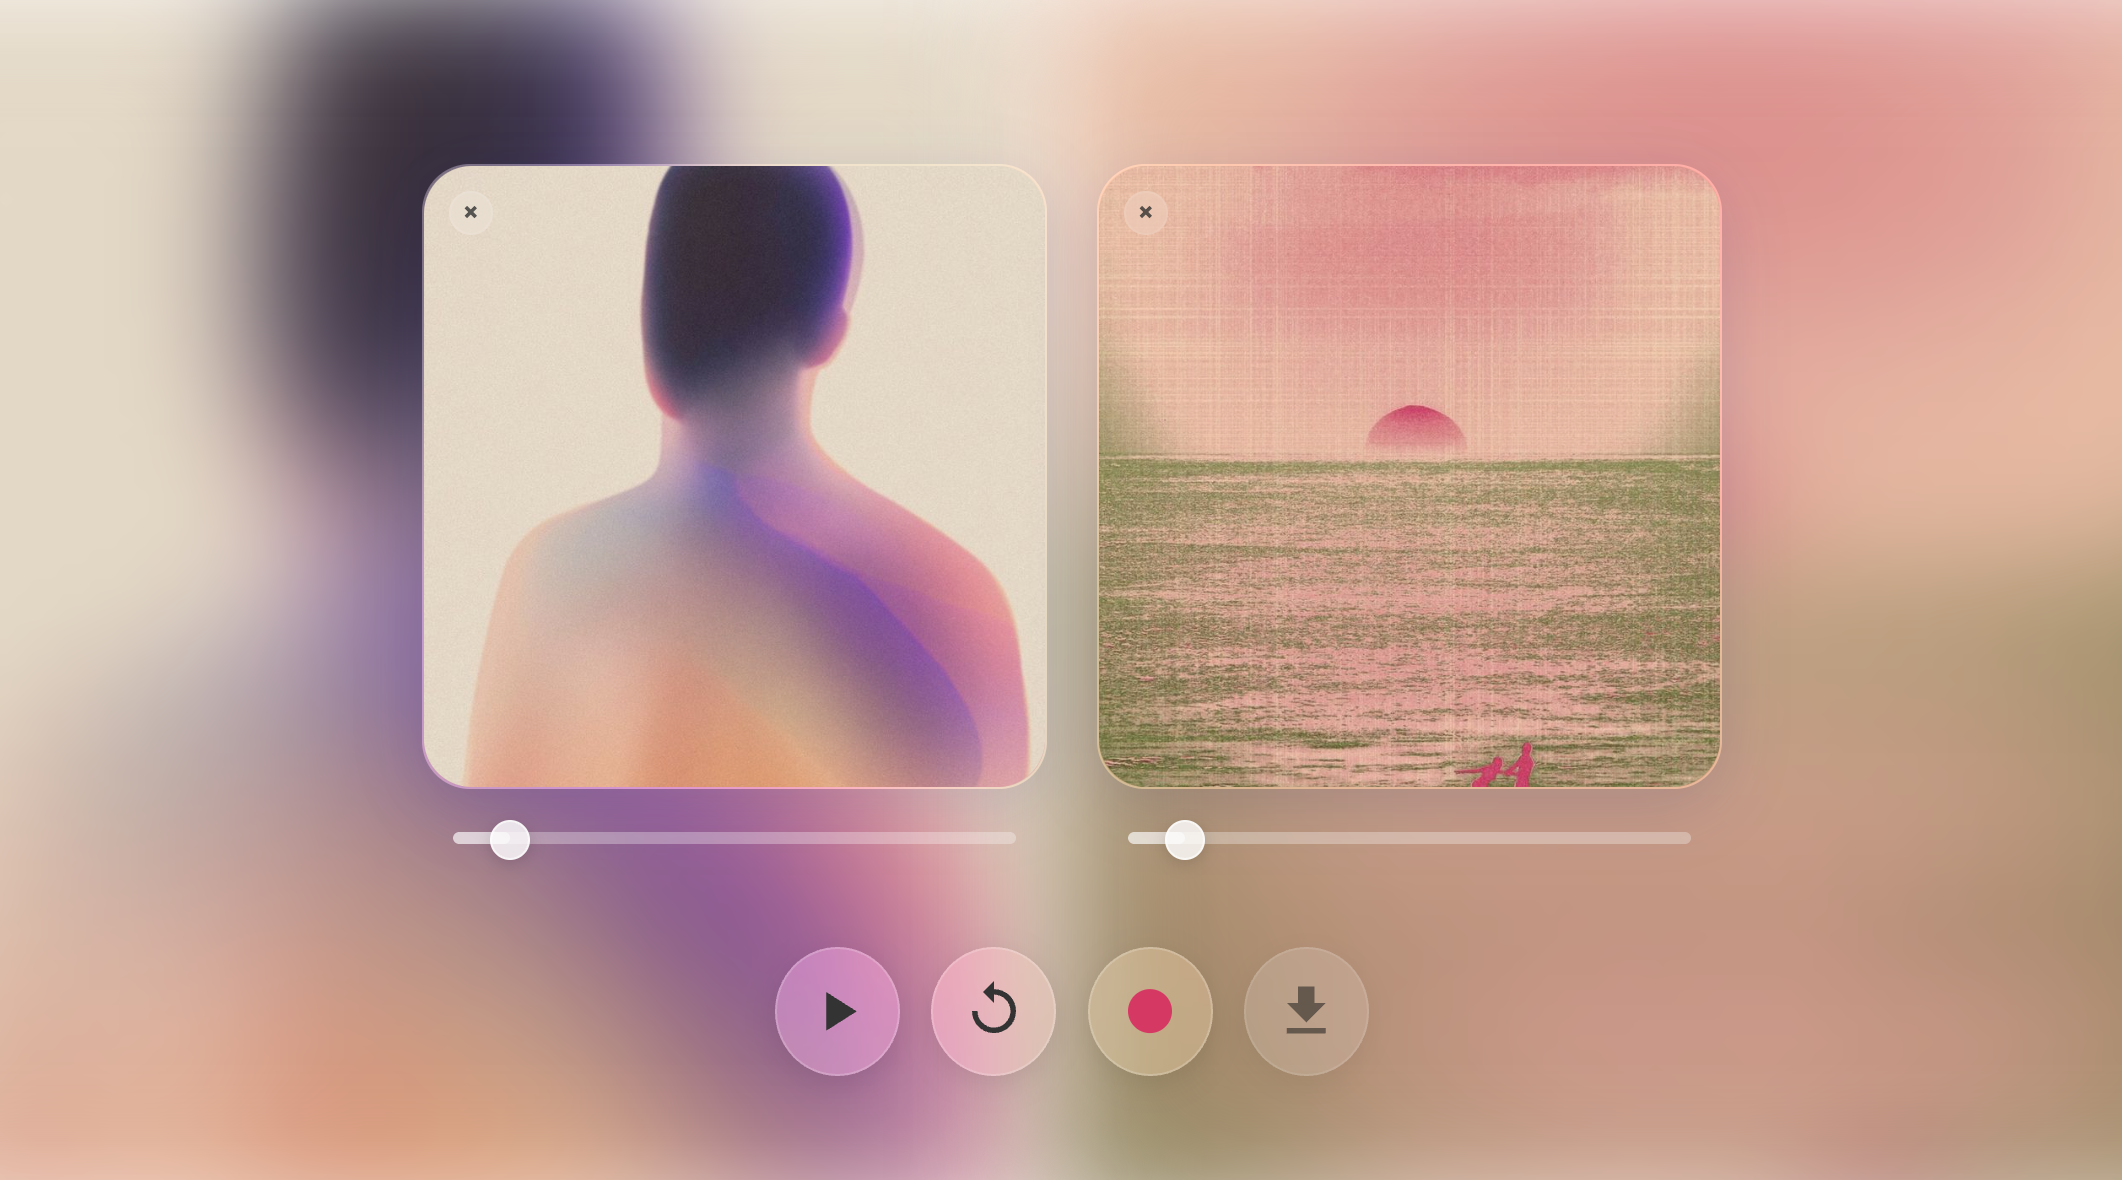
\includegraphics[width=.75\linewidth]{vibesynth.png}
    \caption{Vibesynth.ai, (https://vibesynth.ai/) a tool developed by the author that allows the user to pass images as reference for music generation and control the influence of each. This tool was developed outside the context of this thesis but serves as an illustration of multi-modal inputs for generative AI systems}
    \label{fig:vibesynth}
\end{figure}

\begin{figure}[htbp]
    \centering
    
    % First subfigure
    \begin{subfigure}[b]{1\textwidth}
        \centering
        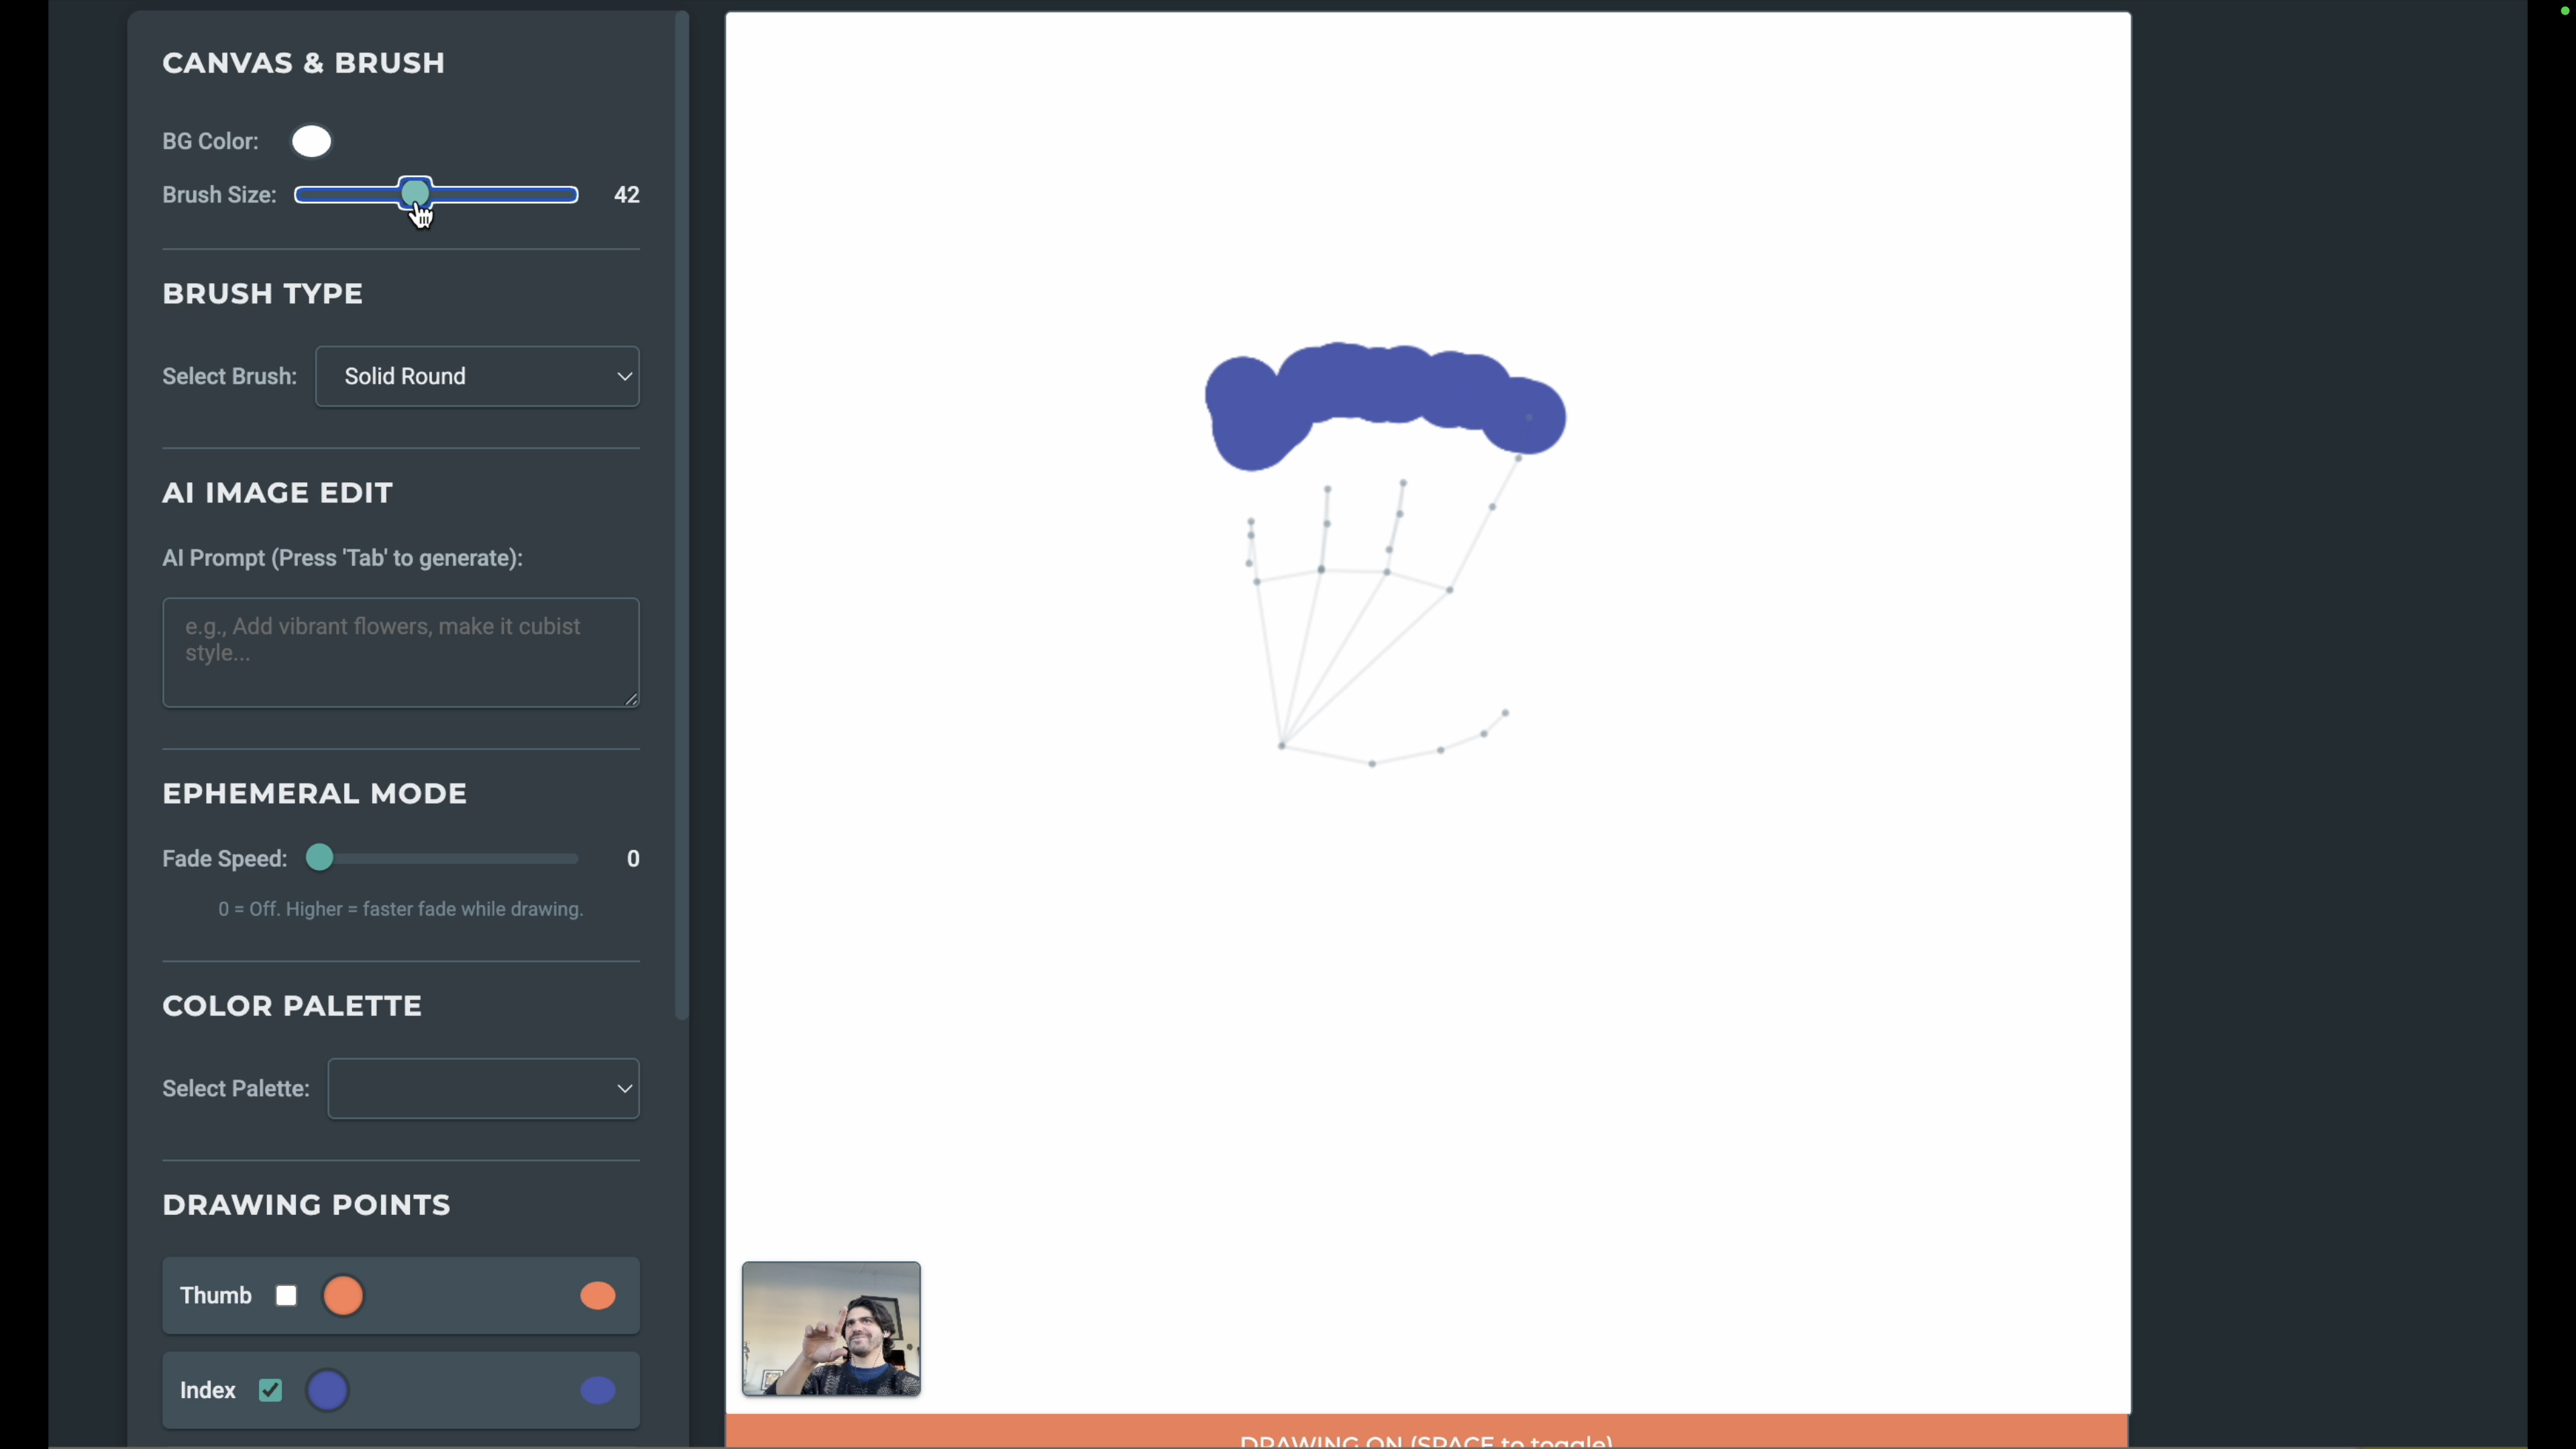
\includegraphics[width=\textwidth]{gesturedraw.png}
        \caption{Prototype interface of gestural drawing}
        \label{fig:gesturedraw}
    \end{subfigure}
    \hfill
    
    % Third subfigure
    \begin{subfigure}[b]{1\textwidth}
        \centering
        \includegraphics[width=\textwidth]{ringdrawing.png}
        \caption{Ring drawing interface}
        \label{fig:ringdrawing}
    \end{subfigure}
    
    \caption{Interface prototypes for gestural interaction system}
    \label{fig:combined_interfaces}
\end{figure}

\begin{figure}
    \centering
    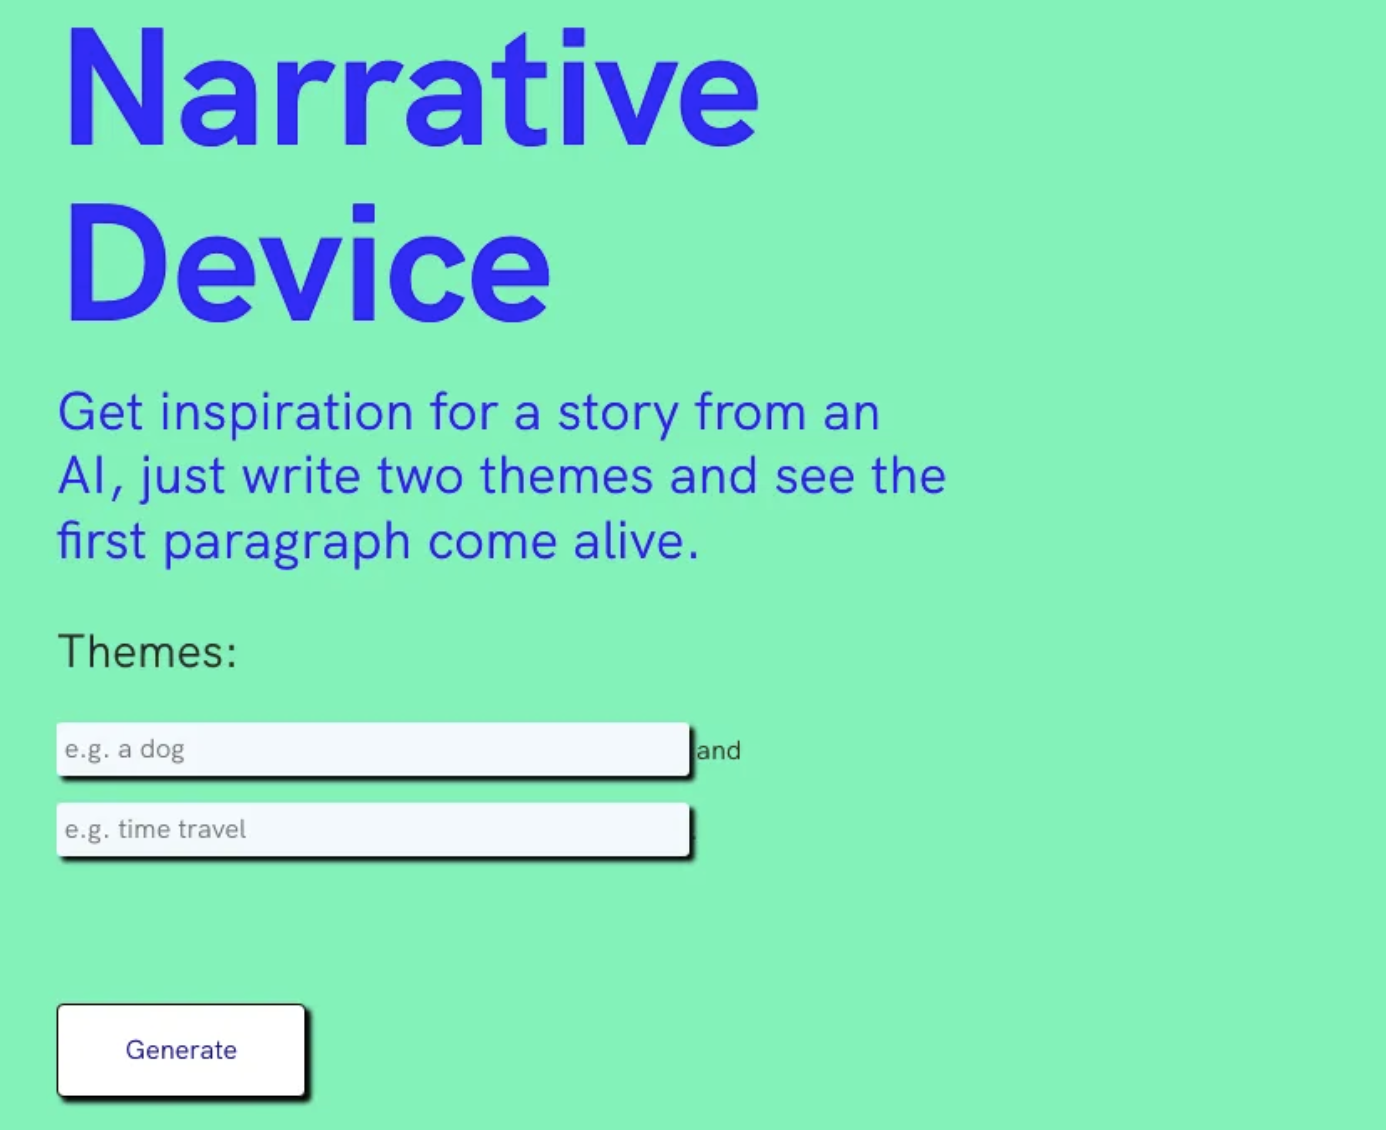
\includegraphics[width=1\linewidth]{narrativedeice.png}
    \caption{Enter Caption}
    \label{fig:enter-label}
\end{figure}

%%%% END EDITING HERE

\subsection{Leaning into the medium and dialogic interaction}

- This warrants here a question related to the dialogic relevance of this process. As I have argued earlier, a crucial element of dialogic interaction is mutual influence. And this is the ultimate objectve of a co-creative interaction, producing something different from what each of the actors would have produced alone. Each induces shifts in perspective and new directions in the other. 

- By leaning into the weirdness of the generative AI medium, unique Ai contributions can be integrated, and new possibilities enabled, difficult to achieve with other means. 

- This was the explicit intention of our impossible photography practice described in Chapter 5: telling visual stories of the subjects not possible through other means. 

A question that emerges here is: how dialogic is the process? 

It helps the user mantain involvement in the process. 
More importantly, I have discussed at length how mutual influence is a core part of dialogic interaction. Not only the user influencing the system and controlling it. 

But also being influenced by it: stimulating a shift in perspective, and leading to a new direction. 

This is ultimately the intention of co-creativity: that the produce is didfferent from what the human would have created otherwise, understood as the output of creative contributions from both human and machine. 

However, it is true that this still leaves things unresolved from a ractical perspective. Users often have specific intentions in mind. 

While generating these shifts in perspective, and leaning into the weirdness and unpredictability could be useful in divergent stages of the process, convergent stages require more granular control, moving towards an output. 

- By leaning into the weirdness of the generative AI medium, unique Ai contributions can be integrated, and new possibilities enabled, difficult to achieve with other means. 

- This was the explicit intention of our impossible photography practice described in Chapter 5: telling visual stories of the subjects not possible through other means. 

- However, as I discussed in that same case study, there is a trade-off. to leverage these tools, it is needed to move from divergent stages towards convergence by refining outputs. 

- And this remains a particular challenge with generative AI tools. 

- There is a tradeoff between surprise and control. 
- A core balancing act in interaction design for co-creativity. 

One one hand, this could mean that some co-creative tools may simply just be used as part of ideation and divergent process. A tool like Narrative Device does not pretend anything else. It is meant to stimulate a beggining, and to serve as a kickstart for users' creativity. 

But other tools perhaps are framed as participating in a more complete creative process, from ideation to convergence, or perhaps are framed to be more of a convergence tool. 

In this case, control and steering is important. In the following section, I discuss some strategies to answer this: multimodal inputs and controls, allowing users to train their own models, iteration, communication and having a space to contribute and make changes at the artefact level. 


\subsubsection{Control through training, multimodal inputs, iteration and communication}


So while in the previous section I discussed the value of leaning into the unpredictability of the medium, here I discuss the importance of offering a level of control. Indeed, it may be the case that this is a trade-off that co-creative tools need to address: to what level does the system offer granular control and to what level they lean into the unpredictability of it. This is perhaps something left to the user, and some tools already offer different controls for levels of creativity. 

The case study in Chater 6 offers an illustrative example of the importance of balancing this, and adhering to a control. In that case, we had two specific control problems. On one hand we wanted to control the style of the generation. We also wanted to control the scene. And we also wanted to control the likeness of the person generated. To achieve this, I explored a variety of workflows and tools. 

We arrived at the the final one, which involved: 

- Using generative tool MidJourney to generate the scenes. This system was better suited at generating high quality visuals and adhere more closely to ouor prompts, being able to have a greater control of the generated scene. 
- However, we were not able to generate the subjects, like the Prime Minister in Australia to a good enough likeness. 
- So as a result, we needed to train a Stable Diffusion model using a dataset of images of the Prime Minister. 

- We iterated multiple times, seeing the results of the model, and often wnriching the dataset, curating and removing images form the trainning set, to align it more with our intentions and the likeness. Arguably this is where we spent the most time. 

With this, we needed a way to connect the two. 

Using the scenarios geerated in MidJourney, to place our subjects within this. 

- We used an image-to-image workflow, which allows to pass an image as reference, which can extract the depth, pose, edges and colour palette of a reference image, and generate the subject in it. 

As the editorial team from the magazine described: "We trained it [Stable Diffusion] to become a specialist in how our Power listers look. Midjourney is more of a generalist; you can’t control its inputs, but it’s better at creating beautiful settings and scenes."

"That is why Beor used Midjourney to create the various environments in which we wanted our Power listers to appear – negotiating with aliens, practising kung fu a la Bruce Lee. The final step involved Ocampo feeding that environment into Stable Diffusion as a reference image, and asking it to include the various avatars he’d already built."


There was an iterative process, curating the dataset, and training multiple models until we arrived at one we liked. 


"Ocampo then trained an AI called Stable Diffusion to generate an avatar of each person. The AI learnt the features of our subjects and got better through trial and error."

https://www.afr.com/politics/federal/what-we-learnt-when-making-ai-images-for-the-2023-power-issue-20230830-p5e0jp

"We trained it [Stable Diffusion] to become a specialist in how our Power listers look. Midjourney is more of a generalist; you can’t control its inputs, but it’s better at creating beautiful settings and scenes."

"That is why Beor used Midjourney to create the various environments in which we wanted our Power listers to appear – negotiating with aliens, practising kung fu a la Bruce Lee. The final step involved Ocampo feeding that environment into Stable Diffusion as a reference image, and asking it to include the various avatars he’d already built."

Similar practices are found in practice. For example, writer Sloan described this as integral to his creative practices experimenting with language models as co-cwriters:

He describes the problem with language modes is that the data they were traine don is extremely boring. 
As such, a large part of the work, reward and consequence stemmed from curating new data to train on. 

He curated a "custom" dataset, consisting of 150GB Pulp Magazine Archives. As he describs this process of finding non-boring datasets is largely where the process lies. 
\begin{quote}
    So, a large part of the work (and fun) of applying the deep learning scenesters’ hard-won technical triumphs to weird/fun objectives is tracking down non-standard, non-boring datasets. For me, decisions about the collection and processing of the text corpus have been more consequential than decisions about the RNN’s design and subsequent training.
\end{quote}

This contempt and frustration with the style of the output of models, particularly those which have fine-tuned and trained extensively to adhere to human preference, have remained a critical point. From my Chapter 4 studies, some participants echoe this sentiment: 


"My main frustration with ChatGPT for writing is that it creates bland, non-passionate work."

While another participant claimed: 

"The writing is incredibly clique (sic), generating very bland writing similar to a motivation quote."


As such, it is becoming a more widespread practice for tools to enable people to train their own models, so they can fine tune their style. This opens beyond the interaction, design interesting question about the authenticity of the work.. 

For example, Leonardo AI LoRA training allows people to train their own models, even though they are fine-tuning an existing Stable Diffusion model. 

Another tool, Exactly.ai, allows people to train their own models bringing their dataset (https://exactly.ai/). Interestingly, this tools allows people to then  upload the model to the platform, making it public and allowing people to use them for commercial purposes, getting a revenue share from their usage. In the platform, users go a verificiation process to verify it is their own work (though it s not exactly clear what thi process entails), which allows them to make the models public and receive remuneration for them. Crucially, they retain copyright of all generated outputs. 



\subsection{Is this dialogic}

Using this strategy (training models on custom datasets) to deal with generative variability and control opens interesting questions about dialogic design. What can these examples telll us about the value of dialogic design? Is this a form of dialogue?

In my conceptualisation of dialogic co-creativity, one of the key elements were mutual understandnig and mutual influence. I argue that when a user engages in the process of curating, and training a generative model with a custom dataset, they are engaging in a dialogue with the system, particularly if there a multiple rounds of iteration of dataset selection and training Importantly, this could be understoof as a process in which the user and the model form a mutual understanding. Indeed many of the approaches involving training a model also involved naming entities with id names, such that the user can use a particular feature or subject in an image without having to extensively describe it in words. Simply they use an identifier that only has meaning in the context of the particular interaction between that user and the model they trained. 
thhis was specifically the case in my Chapter 6, training models of each of the subjects used. Where we engaged in multiple rounds of curating datasets, training models, and naming specific subjects with unique identifiers that triggered the generation of their likeness. 

On another level, this can also be understood as helping the user form a mental model, an understanding of what is the latent space that the generative model operates with. In the absence of this, a simple prompt box with a generic model obfuscates what is behind it. Users come at it, at least partly, blind. When the user curates the latent space t operated with, it gives greater visibility, a known usability principle, of how  the system operates, and how inputs will map to outputs, and how they can better translate their intentions into actions. 

Moreover, this proces can be understood as one of mutual influence. Whereas in the section above, leaning into generative variability and weirdness to induce shifts in perspective is way or inducing AI-to-human creative influence, allowing people to train or fine-tune models can be understtod as a form of human-to-AI influence. Closing the bidirectionality of mutual influence. 

But training or fine-tuning models is not the only way they control can be exercised by the user. Another way is providing the elements that they can work with. For example, in my Chapter 7, the soundscapes were produced from a library of human curted and recorded sounds. The role of the LLM was to drive how these were combined. 

So while we did not train a system (beyond conditioning with prompt engineering) we still curated the outputs of it. 

This was a tasks primarily undertaken by the lead composer and the Uncanny Valley team. They field-recorded sounds from the surrounding environment where the installation would appear in (recall the intention was to turn this environment, or the Opera House building into music). They also composed and recorded sounds in the studio, as well as curated some existing samples and stems to be used. 

This process of curation, of meta-creation was a deliberate decision to mantain compositional agency, to mantain involvement, and ultimately be able to control how the final soundscape would sound like. 

As Justin Shave, shared illustrating how the balance between leaning into the generative power of a system and mantaining a authorship over it through the selection of sounds (and definition of the bounds wiithin which it operated it), the lead composer of the project claimed: "We don't know how the Opera House is going to sound. It's going to be a surprise!" but "I'm going to make it sound good!"

This example suggests further inquiry into how we can provide users with control over the output, to mantain their involvement, and helping them navigate the challenge of generative variability through and adaptive process. 

Another way to provide controls beyond text is by allowing users to express intentions by showing, not telling.

Ealrier I discussed how it is difficult to articulate tacit knowledge such as style and expertise, and convey nuanced things in interfaces such as text-to-only, and this is often recognised as a limitation of generative AI. It is often very difficult to express certain creative intent, or control expressively using limited request based or command-based interfaces. For example, a study by Park et al. \cite{Park2024-gw} titled "we are visual thinkers, not verbal thinkers!" analysing how designers use generative AI tools found their main struggles was to express visual things verbally.


In the case of image generation, interfaces that allow for using image references are one such approach. For example, in Chapter 5 I described how we used some images as reference to drive the generation of our final outputs, as shown in figure \cite{fig:ai_generation_workflow}}


\begin{figure}[htbp]
    \centering
    
    % First subfigure - Control network workflow
    \begin{subfigure}[b]{\textwidth}
        \centering
        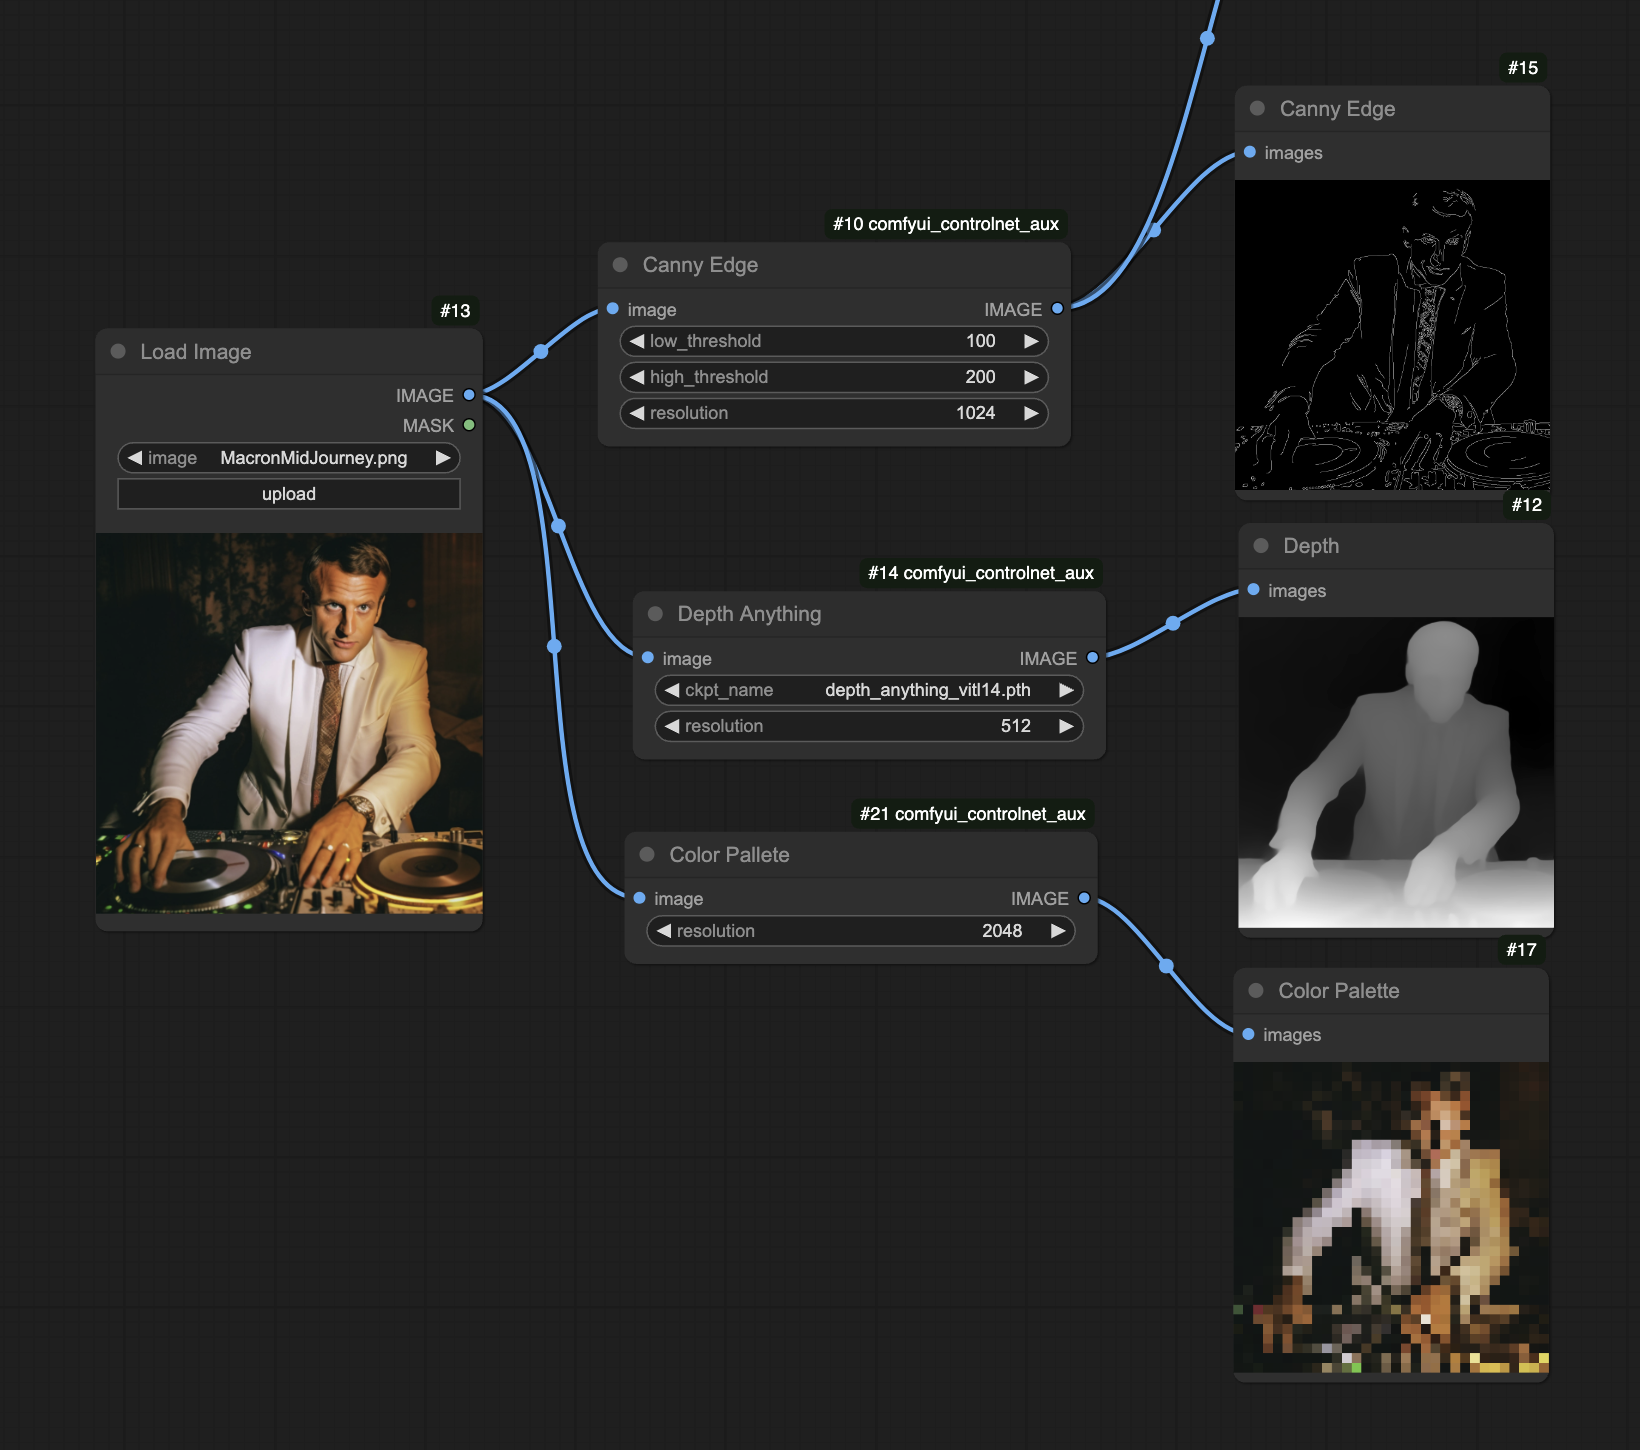
\includegraphics[width=0.9\textwidth]{controlnetworkflow.png}
        \caption{Workflow used to extract characteristics of an image used as reference. The reference image was generated in a software that better aligned with the aesthetic intent.}
        \label{fig:controlnetworkflow}
    \end{subfigure}
    
    
    % Second subfigure - Input/Output comparison
    \begin{subfigure}[b]{\textwidth}
        \centering
        \includegraphics[width=0.9\textwidth]{inputoutput.png}
        \caption{Using a generated image as reference allowed us to achieve the desired result}
        \label{fig:inputoutput}
    \end{subfigure}
    
    \caption{AI image generation workflow showing the process of extracting visual characteristics from reference images and applying them to generate target subjects with desired aesthetic qualities.}
    \label{fig:ai_generation_workflow}
\end{figure}

But often designers and creative do not work with a single specific reference: they often want to express a mood, or a general aesthetic. For example designers often curate moodboards and richer board that contain colour palettes, references and ideas, which they use to then create. In a study by Peng et al. \cite{Peng2024-tr} the authors described the creation of an interface that allows designers to curate moodboards, including colour palettes, images, ideas. When testing it with designers, they found it allowed them "explore and express themselves more effectively" than text-to-image tools. 

\begin{figure}
    \centering
    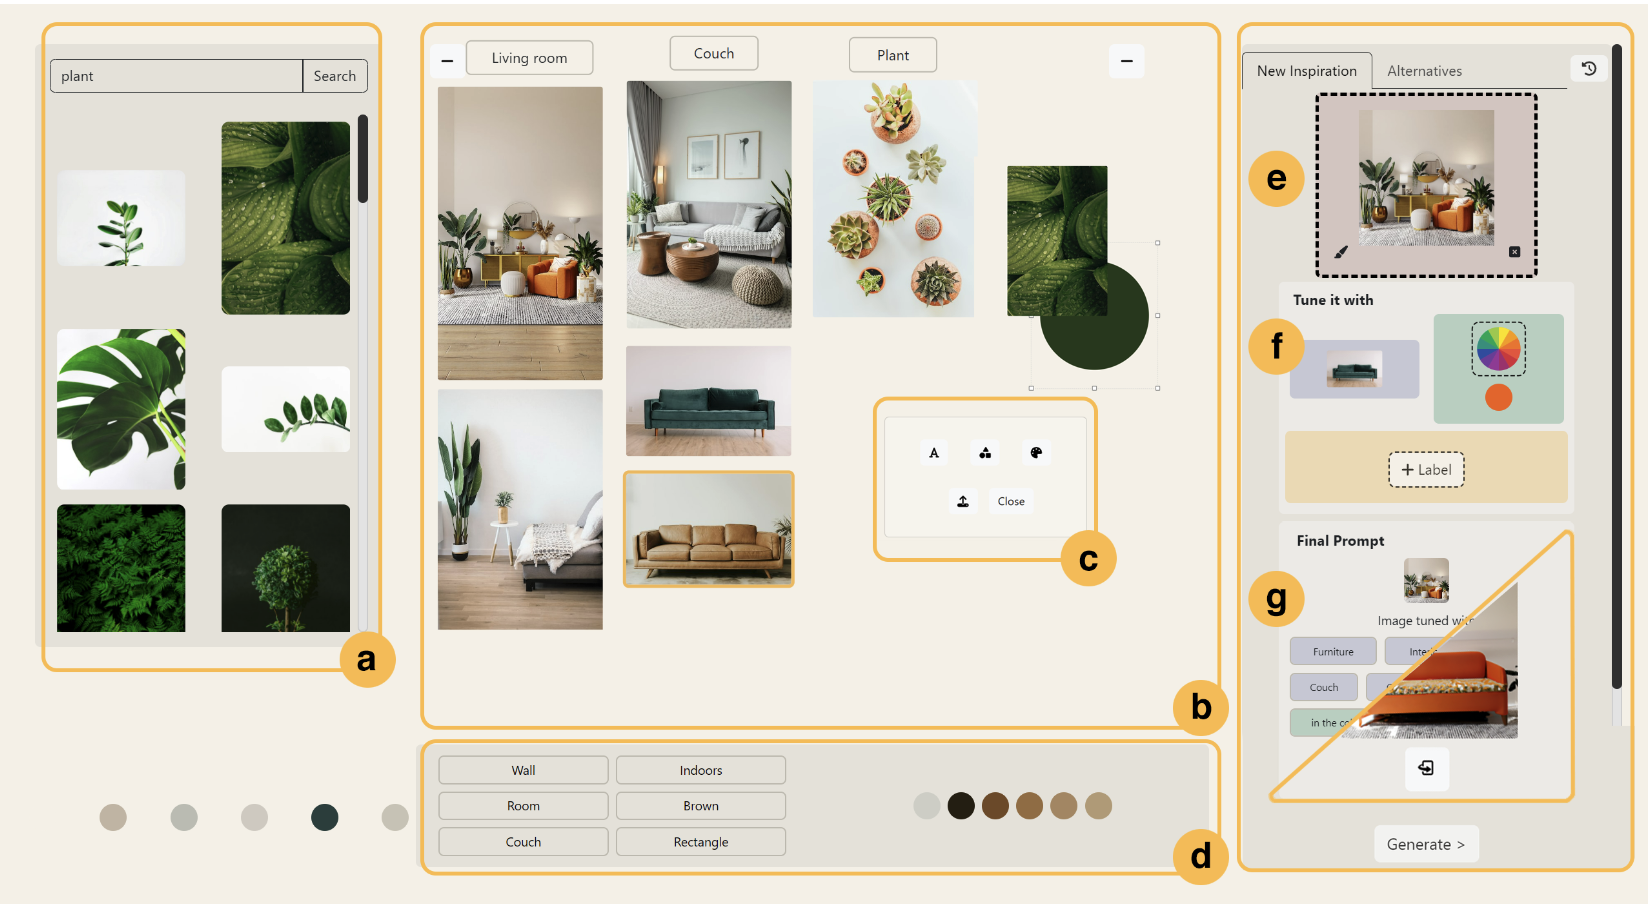
\includegraphics[width=1\linewidth]{designprompt.png}
    \caption{DesignPrompt: a moodboard tool by \cite{Peng2024-tr} allowing designers to search images compose multimodal prompts with images, colors, semantics and text and "finely tune their intentions"}
    \label{fig:enter-label}
\end{figure}

In other modalities such as music, expressing intent verbally may be even more difficult. As a prototype speculating on the possibilities of more tacit interfaces for expressing intent, I build Vibesynth.ai is a tool that lets the user input two images as a "vibe" to generate a soundscape. The images get passed to a visual language model that then is tasked to generate a description of the image, and then this gets passed as a prompt to a music generation system. This process is similar to the process described in Chapter 6, where we used an LLM to generate a description of data, and then used that to semantically drive music generation. In this case, however, instead of using data, it is music. 

This may not be practical when a very specific musical need, such as generating something in a particular key with a particular tempo or instrumentation, but the intention here is to provide a more expressive interface that could capture, at least partly, something more difficult or cumbersome to express in language. While the images are still converted to language and language is being used to drive the generation, the user simply inputs images. This experiment was conducted as a speculative experiment exploring some of the ideas described here emerging towards the end of the PhD, and as an extension of the case studies describes in Chapter 7. In order to make claims about how well this system may help users expressivelt convey musical intent, studies would be requires that were not performed. But the reader can test for themselves at vibesynt.ai

The point here is that generative artificial intelligence may open possiblities for different creative operations, and novel semantically rich translations between modes, rather than drier mappings. 

From a dialogic perspective, this process can be understood, to some degree, one of facilitating translating intention into action, when the intention is difficult to put into words. 

To what degree is this achieved is to be seen, and ultimately, it may be the case that the most dialogic interfaces, allowing for the most alginment between intention and action, are hybrid interfaces that combine text, conversation with rich modalities, allowing the user to shift back and forth between expressing things in language and pointing at things, much like humans in creative activities do. 

When two musicians working together cannot express something in language, they simply just play. 


\subsection{Iteration, Exploration and Convergence}

Another way to deal with generative variability and lack of control is iteration: often the outputs will not be good at the first generation, but through iteration they could be refined towards a final desired outcome. However, this is notably difficult with generative AI tools and it is often recognised as a key limiitations for the creative usability of these tools. 

As an iluustrative example, see in figure \ref{albo_series}. We had liked one of  the outputs shown in the left, but wanted to change the subject to be smiling. However, by trying to change this, just with a single word change in the prompt, and exactly the same setting, the image changed significantly. While the positions and general scenne was retained, a  sut jacket as added, and the overall contrast of the image changed. Indeed, this often recognised as one of the main limitiations of generative AI tools, particularly int the context of professional design practice \cite{Park2024-gw}


\begin{figure}
    \centering
    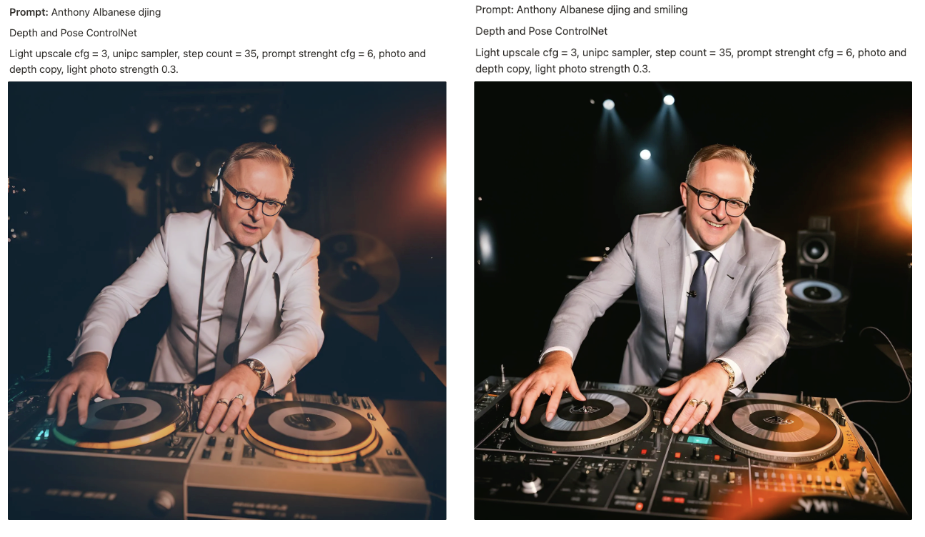
\includegraphics[width=1\linewidth]{alboexperiments.png}
    \caption{Screen-grab from my experiments log from the AFR case study, fixing some parameters while varying others. This example illustrates the difficulty of iterating with generative models. The intention was to change the facial expression of the subject, adding a single word to the prompt while using ControlNets to condition the generation. However, clothing was added, and the brightness and contrast of the image changed as well.}
    \label{fig:albo_series}
\end{figure}

So while in some cases, partculary image models, the lack of refinment and iteration is simply a technical problem, though emerging models like Kontext and gpt-image-1 provide a better level of refinement while mantaining other parts consistent, in many cases iteration can be addressed from interaction design, even if the base models do not fully afford this functionality. 


Emerging commuities of practice provide "guides" to navgate the latent space \cite{Smith2022-dm}. And this navigation largely involves being able to track how inputs map to outputs, in controlled experimentation. Throughout my own practice, particularly in case studies 5 and 6, I kept journals about how some prompts mapped to outputs, some of the experiments are detailed in Chapter 6. 

In retrospect, it is clear that interfaces that allowed me to do this would be creatively useful. 

For example, one can imagine a tree-like interfaces that allows users to see branchings of inpputs and outputs, and mantain rich histories, such as Resnick et al. \cite{Resnick2005-fs} recommend in their Design Principles for Tools to Support Creative Thinking. An example of a prototype imlementing is shown in figure \ref{fig:linus}. And this sort of record-mantaining excercise oof the iterative process may be useful to form mental models of the system. And this may be a crucial point to design for: the forming of mental models of a system

Other tools allow, for example, to combine and "remix" outputs in an iterative process, that may allow the user to take elements they like from an output and combine it with another \cite{Zhou2024-vp}, or branching interfaces for. 

Gradual refinement remains a more challenging task, particularly in image domains, but some new models are making significant progress in that domain. For example, a tool like gpt-image-1 is already letting users modify aspects of images, to varying levels of success, though they degrade over multiple iterations. In other domains, like text, the opportunity to address iteration and refinement may be more immediate. For example, as I will discuss below, people have often complained that Chat based interfaces, with a single stream of messages is limited for iteration. 

For example, in the case of writing, when describing limitiations with ChatGPT, one particulat described that the process writing with it "feels somewhat random and not as iterative."

While another claimed: 

"Chatgpt will always rewrite the entire passage to change just one paragraph and it is harder to work on one text as input as i (sic) often need to scroll back up to see it or continually copy and paste it. "

While another described:

"I’ve felt frustrated because it’s gone in the wrong direction and then requires a lot of input from me to put it on the track that I have in my head"

This was the motivation for my prototype described in Chapter 4, where I provided a collaborative space, separate from the chat window, which mantained state of a piece of writing, that both the user and AI could iterate on. I will discuss this specific interaction design strategy in more detail in a sunsequent section, along with what it may entail in other aspects of the co-creativity such as involvement and conflicts of territory. 




\begin{figure}[H]
    \centering
    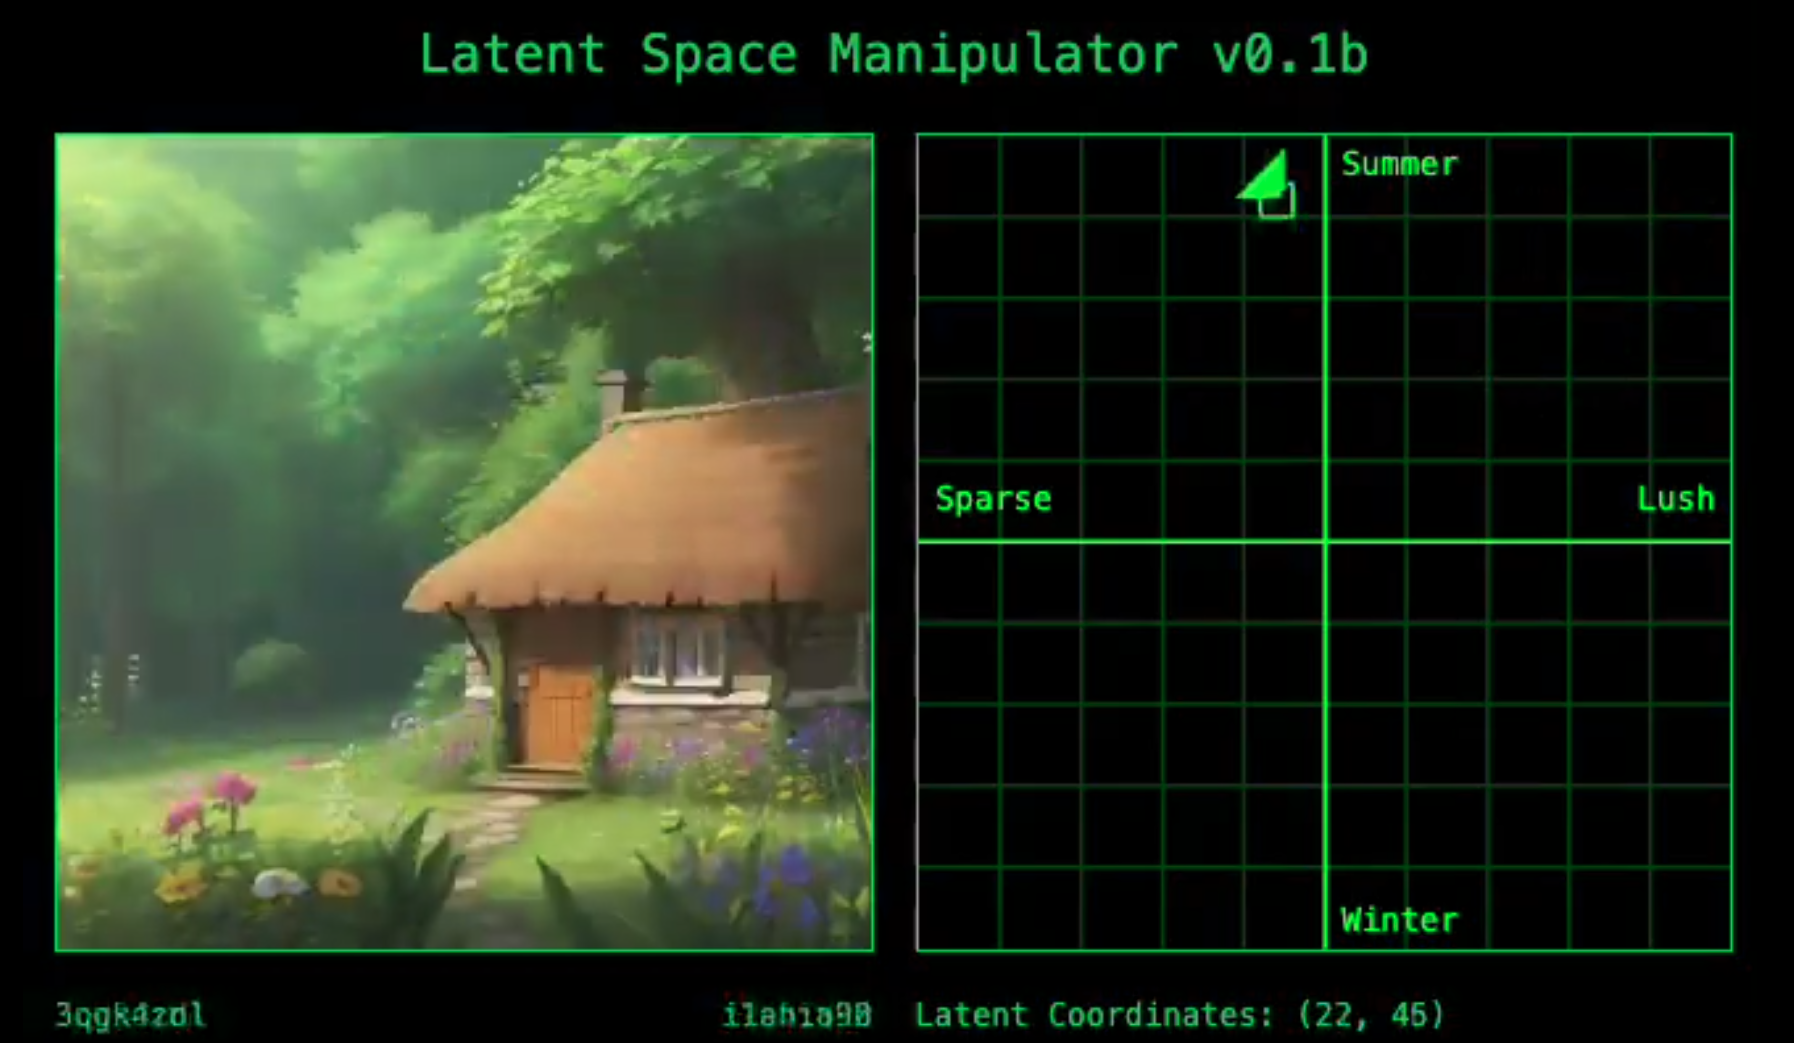
\includegraphics[width=0.8\linewidth]{latentspacemanip.png}
    \caption{Prototype by Michael Feldstein for latent space manipulation, allowing for more intuitive exploration.}
    \label{fig:feldstein}
\end{figure}

\begin{figure}[H]
    \centering
    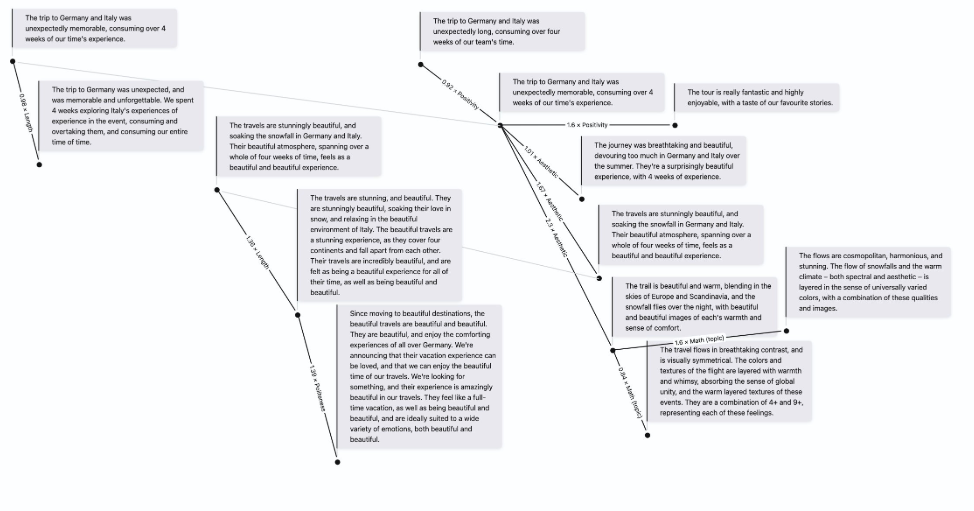
\includegraphics[width=0.8\linewidth]{linus.png}
    \caption{Linus Lee's experimental interface for exploring creative possibilities.}
    \label{fig:linus}
\end{figure}



\subsection{Opportunity 4: Use conversational spaces to build mutual influence and understanding, not just instruction following}

Today, conversational interfaces are the main form of interaction with LLMs, but that was not the case at the beginning of this thesis. Interaction with LLMs and indeed most generative systems happened through instruction-response, one-shot modalities, or autocomplete functionalities. So the question of how well these systems could engage in bidirectional communication and how this could improve co-creativity was largely an open one.  My early experiments in Chapter 3 investigated this. This involved repurposing an autocomplete-based LLM into a co-authors that could engage in conversational dialogue. A key interest was to investigate whether models could switch between discussing creative goals and performing creative tasks in one single thread. These explorations showed a nascent capacity for this.


\begin{figure}[H]
    \centering
    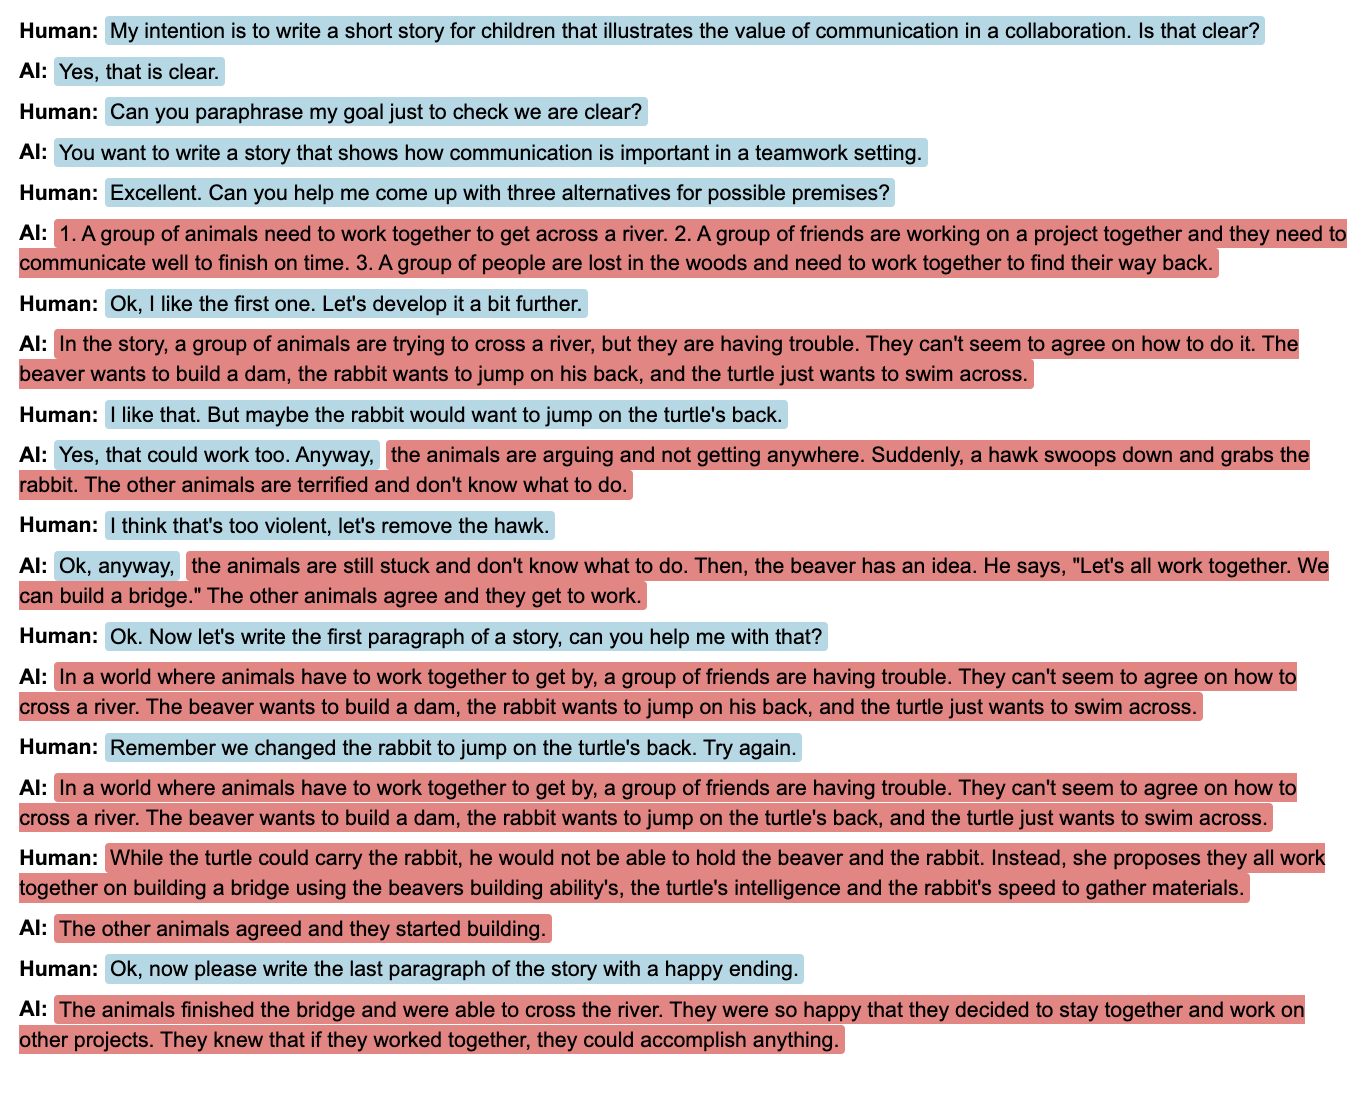
\includegraphics[width=1\linewidth]{transcriptgenchi.png}
    \caption{Transcript of an interaction with GPT-3 before the launch of ChatGPT, showing early potential for dialogic exchange.}
    \label{fig:genchi_transcript}
\end{figure}

A few months later, ChatGPT was launched, confirming the potential of bidirectional communication in terms of co-creative usefulness, as reflected in its wide adoption across creative activities. 

However, whle the wide adoption of conversational and dialogue based interfaces have illustrated, in practice, the potential of dialogic interaction. However, it has also highlighted it's challenges in terms co-creativity, particularly in the case of writing. 

- It still puts user in a requester role, as it allows them to mostly engage about the writing, providing requests, etc, rather that at the level fo writing. And with this, it limits the involvement o the user at the writing level. 

- This can lead to Erosion of skills, limiting the confidence and ability of practitioners to turn their intentions into outputs, and it turn, their creative agency. A growing literature finds that overreliance on LLMs can lead to skill loss \cite{Heersmink2024-mk, Rafner2021-tm}. Gerlich found that overreliance on AI for writing tasks is linked to a loss of critical thinking skills \cite{Gerlich2025-as}. A recent study by Lee et al. \cite{Lee2025-dw} found that the use of generative AI in knowledge workers was linked to less cognitive effort and reduced self-confidence. This is particularly concerning for creative agency, as creative self-efficacy, defined as confidence in one's creative ability, is a crucial determinant of creative achievement \cite{Tierney2002-xp}. 

In a recent preliminary study by Kosmyna et al. conducted at MIT \cite{Kosmyna2025-cm}, reseachers explored the neurological effects of engaging in a creative task using EletronEncelography (EEG). They compared participants using no tools, using web search, and using ChatGPT. They found that participants using an LLM via a chat-interface they showed significantly lower levels of brain connectivity, brain activity patterns signaling under engagement with the task, they struggled t quote their own work, and reported lower levels of ownership of the essay. 

Involvement and immersion are crucial aspects of the creative process \cite{Amabile1996-pt, Csikszentmihalyi1997-ui} and an important dimension of analysis and design in co-creative systems \cite{Davis2016-te, Cherry2014-ty, Rezwana2022-ui, Clark2018-yf, Lawton2023-gd, Yuan2022-kb, Li2024-yh, Kantosalo2015-pk, Resnick2005-fs}. Generative AI offers new possibilities to realise more powerful and useful co-creatve systems. However, paradoxically, their creative power and capability can lead them automate most aspects of the process, providing a path of least resistance to the user, leading them to become less involved. 

Brian Eno's sentiment provides a valuable illustration: 

\cite{Eno2024-rj}:
\begin{quote}
"In my own experience as an artist, experimenting with AI has mixed results. I’ve used several “songwriting” AIs and similar “picture-making” AIs. I’m intrigued and bored at the same time: I find it quickly becomes quite tedious. I have a sort of inner dissatisfaction when I play with it, a little like the feeling I get from eating a lot of confectionery when I’m hungry. I suspect this is because the joy of art isn’t only the pleasure of an end result but also the experience of going through the process of having made it. When you go out for a walk it isn’t just (or even primarily) for the pleasure of reaching a destination, but for the process of doing the walking."
\end{quote}

However, research also shows this is largely mediated by interaction design \cite{Kim2023-wt, Essel2024-qc}. 

\subsection{Opportunity 5: Separate Collaborative Spaces}

In order to address the above this thesis I found that a separate space to the conversational space where users and AI can both collaborate in the action space, interacting through the creation and not only through the creation. 

As discussed in Chapter 4, this lead to users reporting the AI did most of the work less ofte and reporting higher level of involvement and agency. I did not measure satsfacton in a Likert scale, but these responses suggest a differential experience. 

Take the case of a participant in my Chapter 4 study, who used the Chat-only interface (Vorges) tool to write:

\begin{quote}
"[it] made me feel like I was cheating somehow. It does not feel like my work, even though I gave all the ideas. Also, I believe there is satisfaction in putting a lot of effort/dedication/patience into something. Vorges made everything so simple, fast, and easy that it felt artificial and no real satisfaction came as a result."
\end{quote}
Another one using the same interface described: 

\begin{quote}
I find them to be very interesting, and useful tools in getting a job done quickly, but at the cost of loosing a sense of individuality. 
\end{quote}
Compare this with a participant interacting with the Chat + Editor interface:

\begin{quote}
"I really-really enjoyed writing this. I even had a deep moment of reflection, my writing was nostalgic and sad, but I was able to use AI to steer it in the right direction, it gave me confidence that I was also writing with correct grammar and spelling, English is not my first language and while I am proficient, I can still use proofreading to ensure good quality, this tool helped me with it." (P4 Common AI)
\end{quote}
Others shared this perspective:
\begin{quote}
P9 shared: “I liked how my original ideas were still retained, and AI was used to complement my intentions. It forced me to put in some effort and do the majority of the work.”

P22 emphasized: “It adds an element of working together, which I think is the moral problem with current AI tools—they often seem like they’re doing all the work.”
\end{quote}


A participant highlighted the limitations of ChatGPT, comparing it with an AI co-writer integrated within a text editor:
\begin{quote}
P5 said: “It can just be a bit clunky having a separate document to then copy, paste, and edit in [in ChatGPT]. This made it super seamless being in the one program.”
\end{quote}

While another participant claimed:

\begin{quote}
“ChatGPT will always rewrite the entire passage to change just one paragraph, and it’s harder to work on one text because I often need to scroll back up or continually copy and paste it.
\end{quote}


\begin{quote}
Also takes a lot of effort to get it to change a sentence or something that you don't like.
\end{quote}


The simple idea of adding a shared editor next to a chat window to address this was the core of my Chapter 4, and it proved effective in increasing user involvement.
\begin{figure}[H]
    \centering
    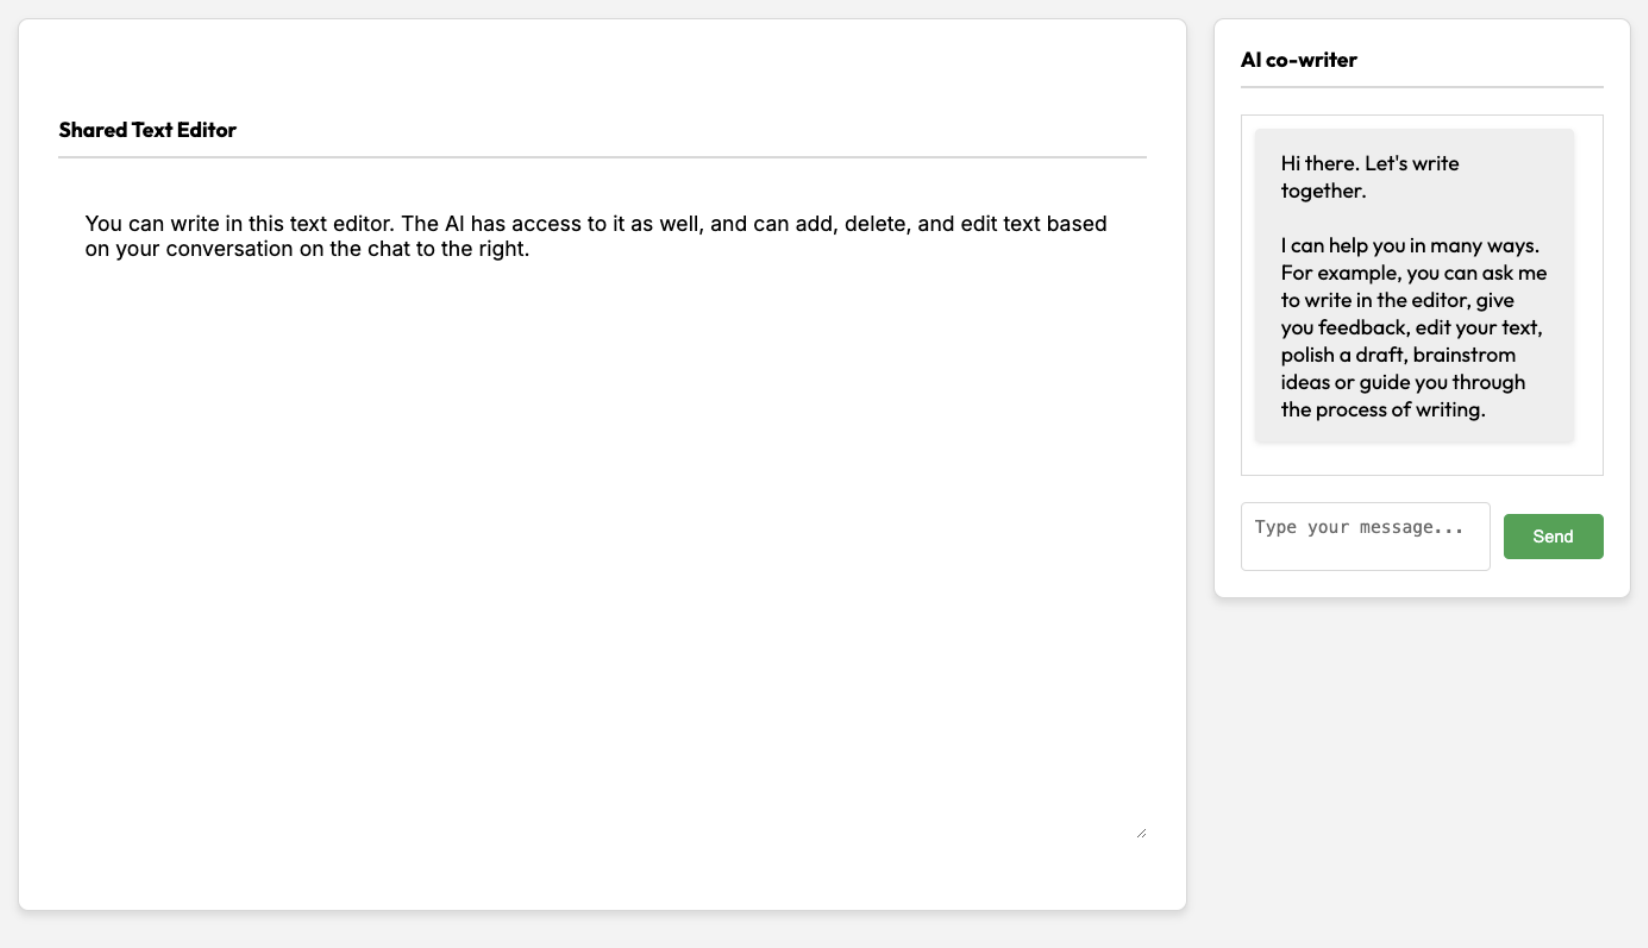
\includegraphics[width=1\linewidth]{sharededitor.png}
    \caption{The shared editor prototype, combining a chat with a direct manipulation space.}
    \label{fig:shared-editor}
\end{figure}

Participants reported more agency: P18 said, “It was much better than ChatGPT. I enjoyed how it gave me a lot more agency.” P12 remarked, “I really enjoyed it; it still let me have autonomy.” 



Involvement is crucial

Sloan, describing his process of creating a text editor powered by an AI described:

\begin{quote}
I am just so compelled by the notion of a text editor that possesses a deep, nuanced model of…what? Everything you’ve ever written? Everything written by all your favorite authors? By your nemesis? By everyone on the internet? It’s provocative any way you slice it.

I should say clearly: I am absolutely 100\% not talking about an editor that “writes for you,” whatever that means. The world doesn’t need any more dead-eyed robo-text.

The animating ideas here are augmentation; partnership; call and response.
\end{quote}

A shared space was used here. 

\begin{figure}
    \centering
    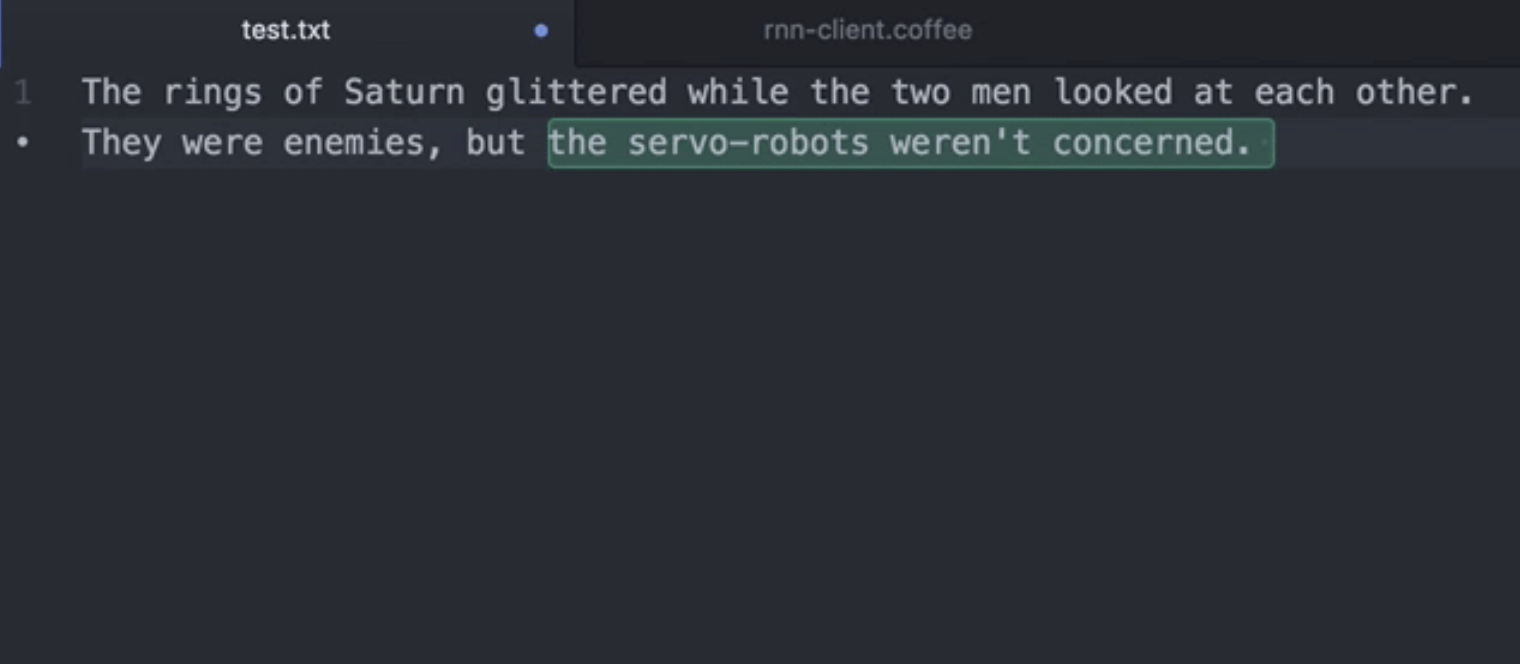
\includegraphics[width=1\linewidth]{rnn.png}
    \caption{Enter Caption}
    \label{fig:enter-label}
\end{figure}


In particular, I refer to managing what has been called conflicts of territory. 

\subsection{Opportunity 6: Manage conflicts of territory in shared spaces}

However, a shared space introduces challenges like managing contributions. Participants expressed this need for better visibility of introduced changes:
\begin{quote}
Participant 11: “When you ask the AI to check your grammar (as I did), it would be good if it told me what suggestions it had made, so I can double check its work easier.”

Another participant commented: “I am unsure as what parts of the text are being edited, in the end I am not quite sure which parts were mine and which ones were edited by AI.”

“Once the tool has made revisions to the original text, maybe it can highlight the key changes that have been made... otherwise I need to slowly read through and identify the changes myself.”
\end{quote}


\begin{quote}
    The one limitation I would say is that if you don't like what the AI as integrated you need to manually remove it from the only source of text you have (the one you are sharing with the AI). Whereas in an AI chatbox, usually you would parse through the original text copy into the chat, and the chat would then spit out a new copy, makes it a bit easier to edit/cut out any additions you don't like.
\end{quote}


This highlights what Buschek et al. \cite{Buschek2021-ks} call "conflicts of territory" in their identified Nine Potential Pitfalls when Designing Human-AI Co-Creative Systems. They describe this as when in a In a co-creative text editor, the AI replaces or destructively edits the content that was written by the user. Or the user makes changes to AI-generated text, but then the AI reverts it. They suggest keeping track of user edits to protect them and to highlight the changes that were introduced by the AI. 

An example of a tool out in the wild that has successfully integrated collaborative shared space with a conversational interface is Cursor. Largely, the value of a tool like Cursor has been that it shares a coding space with a user and whenever the AI is going to generate some suggestions or contributions, it provides the user with the diffs that they can accept or reject. They can also revert and maintain a version control. 

Of course, this adds complexity to the design of the co-creative tool. In the prototype that I built in my chapter four, this was precisely what I focused on when I went from the first prototype to the second prototype. It was specifically being able to manage how the AI introduced edits into the text and even if I didn't go all the way to producing highlights, the intention was that the AI could make direct edits to the level of a single word without having to rewrite the entire text, which may affect or change the text of the user had rewritten. 

To achieve this, I created a protocol that the AI could use to call particular edits within a single text, which is similar to what Cursor does. It uses things like rep and the use of tools within the coding environments to be able to control a specific edit set. 

Shared spaces are important to allow the user and the AI to interact both through and about the artifact. Increasingly, we will begin to see more co-creative systems that are embedded within the editors that people use (text editors, design software, and so on). It becomes important that interaction designers manage the contributions of the AI, manage the conflicts of territory, and enable fluid interactions that are non-destructive. 

It is important to clarify that even if the value that I highlight regarding the shared spaces is that they lead to more user involvement, it does not mean that users are completely involved. In fact, in my studies, both users using the shared space and the chat and users using the chat only both agreed with the statement that AI did most of the work. The difference was that the level of agreement was less in people using the shared text editor compared to the chat-only interface. But in both cases they describe the AI did most of the work. It was just lower significantly lower in the shared space. As the graph \ref{fig:graphsharedspaces} shows, while in the chat-only interfaces participants reported agreed more with the statement that the AI did all the work, in both interfaces the agreement for this statement was high. In other words, even if participants were more involved in the interface that had a collaborative interface, in both interfaces they reported that AI did most of the work. 


\begin{figure}
    \centering
    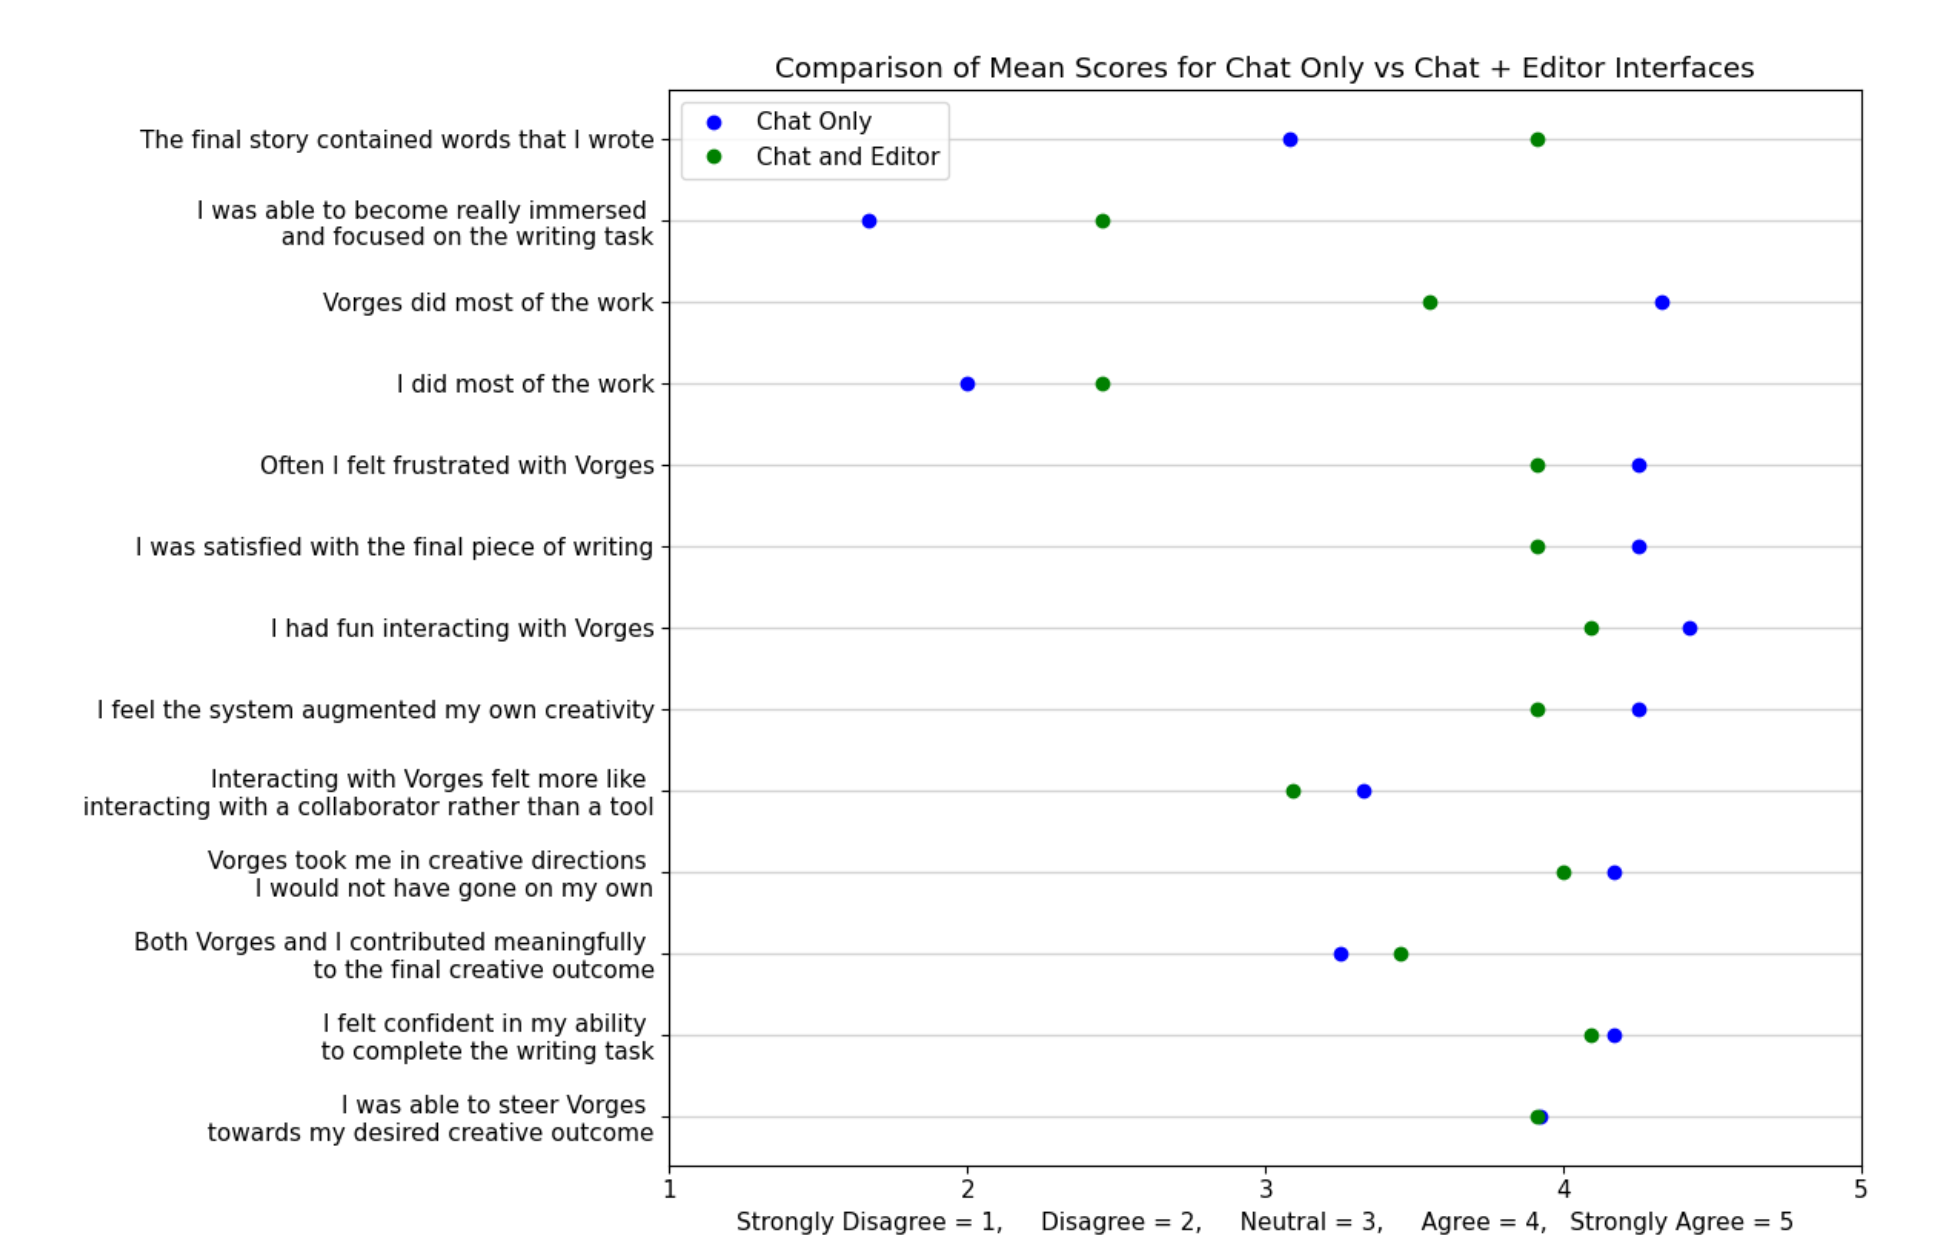
\includegraphics[width=1\linewidth]{graphsharedspaces.png}
    \caption{Enter Caption}
    \label{fig:graphsharedspaces}
\end{figure}

A similar thing happens with Cursor, even if it's integrated within a shared space and is the main coding editor. It carefully manages conflicts of territory through diffs, accept and rejects. By having the AI be able and capable to do the coding, it leads to user to users outsourcing most of the coding. In fact, the vibe coding reference that I reference at the beginning with Andrew Karpathy he was referring to using Cursor, so he was still doing this process of being primarily assuming a role at the intentional level and not at the action level while using Cursor. 

\subsection{The fundamental tension in human-AI co-creativity}

This leads to what I describe as a fundamental tension with designing generative AI-powered co-creative systems. It's the fact that when having a generative AI capable of doing work at the level of a human and more, it provides a path of least resistance that the users may rely on to do the work for them.

While these tools are incredibly capable and they can in theory lead to creativity and to lead to users using them to engage their own creativity and to support their own skills, they also provide a path of least resistance that leads to automation. This is what I describe as a fundamental tension that interaction design needs to address to design generative AI-powered co-creative systems. 



Others have discussed the need to balance automation and human agency \cite{Moruzzi2024-cq}. 

\begin{quote}
    "In this scenario, there is apressingneed toexamine the terms ofthe balance between automation and agency in H-AI interaction to continue reaping the benefts of increased efciency resulting from the automatization of repetitive and burdensome tasks, preserving at the same time the sense of agency, control, and responsibility of users"
\end{quote}

At the same time, the balance goes beyond automation versus agency. Generative AI, as discusses above, has the potential to speed up, help serve as a safety net. And lead into new creative directions. On the other side, it can lead to users becoming less involved, losing valuable skills, a sense of satisfaction, individuality ad authenticity of their work. 


\subsection{Being involved at a higher level of abstraction}


- Lack of involvement at the action space is not necessarily bad
- And assuming roles at the intentional level does not necessarily mean being less involved in the creative process and it may allow users to focus on higher level things

As one participant in my writing described about interacting with Vorges, the AI co-writer: "I like it a lot. I think that it allowed me to focus on the ideas, the plot and the characters even more because Vorges focused on the writing."

- Much like a producer is meaningfully and productively involved by simply providing nudges to the musicians, such famed producers Brian Eno and Rick Rubin have been described doing
- In fact, producer Rick Rubin has been recently engaged with the role of human creativity in the context of generative AI, and particularly, vibe coding. 
- He argues that, indeed, humans will increasingly assume roles similar to the role he has assumed in a prolific career of music producting. 
- In his perspective, human creativity does not risk automation simply because people need another human behind the artwork: they need it to connect. 

- This view contrasts with that of Brian Eno, who, as described above, laments a lack of involvement in the process of actually generating a piece of work. It is not so much about giving the instructions. It is about engaging in the process itself. 

- The question there, may precisely lie in the level of involvement, weather in the intentional space or action space

- An illustrative example is Jason's Allen Opera Spatiale, which he entered as part o a digital art fair in Colorado. 
- The artwork received first place, but generated signficant controversy when it was revealed that it was generated using generative artificial intelligence 
- The artwork was denied copyright by the US Copyright office, and it argued that it was not clear how much was "Allen's work and how much was AI"
- Allen argued he was deeply involved in the process, and he iterated and tested hundreds of prompts, and engaged in the use of digital design software to retouch and modify the image
- For him, the image was generated by him in no way different than other artists using digital software. 
- He was still involved, simply with a different set of tools and creative primitives available to him

- This example begins to highlight that perhaps in generative tools, the intentional and action spaces are blurred: intention is action. 

- Prompting is beggining to emerge as a creative practice in its own right, with large engaged communities of practice developing idyisyncratic and deeply individual approaches to it \cite{Chang2023-tv}

- How does this influence my discussion on levels of involvement? 

- I argue the answer partly lies in the level of dialogic interaction: how much of an iterative cycle of creativity (and co-creativity) with the system is engaged. A person that simply inputs a single prompt, with little thought and perhaps the need to truly express something may be considered less involved than one that has engaged in multiple rounds of iterative, reflective-action to arrive a "single prompt", and with a clear intention to communicate or express something, and where that intention flows into action (output), whatever the means. That is: intention \textit{and} process matter.

- From this perspective, for example, our process describes in Chapter 6 producing visuals for a magazine was highly dialogic: we engaged in multiple rounds of iterating, curating data, training the system, generating alternatives, changing, and compising the tools available to us, even if we did not engage in any form of verbal two-way conversation with the system. 

- In contrast, some participants, in my Chapter 4 co-writing study that engaged with a conversational system, and which describes it as doing "everything" and "all of the work" may be understood as engaging in a less dialogic process, even if that process is seemingly more dialogic from virtue of havig engaged a conversational interface

- The core element for dialogue here is that the iterative building of mutual influence and understanding towards the production of something imbued with a strong intention is the key to dialogic interaction, whatever the means. Interfaces that facilitate this can take many different forms, and conversational interfaces is only one of them, that depending on the conversational design, and how people engage with it, may be more or less dialogic than other interfaces.

\subsection{Creative primitives and humans acting as orchestrators of generative workflows}

- With this framing, let's go back to the discussion on roles, and what it means for humans to assume roles at the intentional space.

- As I argued in the previous section, engaging in intentional roles does not necessarily, by itself mean that humans are less involved creatively: an that process matters.

- What does that mean for a person to be deeply involved in the intentional space. My case studies in Chapter 5 and 6 provide illustrative examples. 

- I argue that the shift in role distribution, and humans assuming roles at the intentional space can be understood as the tendency to move up levels of abstraction, and cognitive promitives in lower levels of abstraction are automated. 

- Nielsen argues that the value for generative artificial in augmenting human intellect lies in that it provides new cognitive primitives to work with, allowing humans to engage in higher levels of abstraction to operate with, much like a calculator does by automating the labouriousness of long division so that humans operate with "long division" as a cognitive primitive that they can compose with others. 

- In the same way, I argue that generative artificial intelligence can provide new creative primitives, automating generative aspects of creative production and allowing users to operate with these creative primitives at a higher level. 

- When the user is deeply involved at this higher level of abstraction, even if they are in an intentional space, their intentional space becomes a new action space, and as such they become more deeply involved in the creative process. 

- Take my example in Chapter 6. In that case, I am prompting the language model to translate incoming data into actions to drive a generative soundscape. On a first reading, this may appear as a lack of involvement at the action space. 

- But with the framing above, I am engaging with this LLM-drive transformation of data to sound as a creative primitive that I operate with, and compose it with others primitives in a generative and non-generative pipeline.

- As such, I become a builder of workflows, and generative models provide creative primitives that become nodes in that workflow. This building of workflows becomes my action space. 

- As Palani described, fro an extensive survey and systematic review, this is increasingly the role describes by creative practitioners engaging with generative models: that of orchestrator, building workflows and connecting things. 


- Increasingly, tools are building interactions and interfaces that accomodate specifically for this type p role, beyond the linear prompt or the conversational interface. For example, ComfyUI is a popular open-source system that allows users to build workflows of different generative tools, connecting them in increasingly complex ways, with users developing personal and idyosyncratic workflows that enable new possibilities, operating with the input-output of different generatve systems across different modalities as creative primitives. 

- Tools like Flora enable similar operations to less technically and coding proficient advanced users enabling a similar workflow building interface targetted at designers and artists. Similarly, Leonardo.ai's workflow building tool and blueprints seel to provide a compositional workflow building tools that give more control and involvement to the user beyond more simple prompt interfaces. 

- And this illumintates a last principle: that of providing visibility to the user about what te creative capacities and limitiations are, which can be described as making the creative primtives visibile, that the user can operate with. 

- In the literature review, I outlined how the effectiveness of human-AI interaction hinged largely on the ability for users to know how the system worked: visibility. When they had a better sense of what was possible, and what was not, they engaged with it in more effective ways, and helped meta-cognivively know which actions (creative primitvies) they should leverage the system for and which ones they should engage with. 

- In my Chapter 4 co-writing studies, a similar qualitiative observation emerged: some users described that whe engaging with these chatbot for co-creating, both with the editor or not, they would benefit for having more clarity about the kinds of things they can do with it, and having direct ways of triggering crtain operations: like prioviding feedback, gemerating text, providing suggestions etc. A srt of direct maniulation GUI that triggers creative action. 

- This points to what Weisz and Nielsen have called intention-oriented interfaces, action oriented interfaces, or outcome oriented interfaces: the creative primitives, the cognitive primitives in co-creatove systems and generative systems are not objects, but processes and actions. 

- Making them clearly visibile, therefore, is of significant important for effective interaction. 

\section{Contribution and Future Directions}
This thesis argued that the current paradigm of human-AI interaction often leads to \textit{severed agency}. The primary contribution is the development of \textit{dialogic design} as a framework to counteract this by more closely aligning intention and action through the principles organised under the dimensions of \textbf{Iteration}, \textbf{Communication}, \textbf{Collaboration}, and \textbf{Integration}. The design principles derived from this research offer concrete guidance for building effective co-creative tools that maintain human agency and allow people to leverage the potential of generative AI.
